\documentclass{article}
\usepackage[utf8]{inputenc}
\usepackage{hyperref}
\usepackage{amsmath}
\usepackage{amssymb}
\usepackage{amsthm}
\usepackage{graphicx}
\usepackage[ngerman]{babel}
\usepackage[T1]{fontenc} %Umlaute in label
\usepackage{xcolor}
\usepackage{enumitem}
\usepackage{framed}
\usepackage{float}
\usepackage{txfonts}
\usepackage[parfill]{parskip} %No indentation



%Start counting from 0
\setcounter{section}{-1}

\theoremstyle{definition} %Make text non cursive
\newtheorem{define2}{}

\newcommand{\Topo}{$(X,\mathcal{O})$}
\newcommand{\Toporef}{\hyperref[Topologie]{Topologie}}
\newcommand{\Toporeflong}{\hyperref[Topologie]{\mbox{topologischer Raum}}}

\newcommand{\listbsp}{\renewcommand{\labelenumi}{(\arabic{enumi})}}
\newcommand{\offUm}{\hyperref[offen]{offenen} \hyperref[Umgebung]{Umgebung}}
\newcommand{\pihalf}{\frac{\pi}{2}}
\newcommand{\Rtwo}{\mathbb{R}^2}
\newcommand{\Rthree}{\mathbb{R}^3}
\newcommand{\aeGebiet}{\hyperref[abgeinfachGebiet]{abgeschlossenes einfaches Gebiet}}

%Custom Environments
\newenvironment{titleDef}[1]{\textbf{#1}\\\noindent}{}
\newenvironment{rawDef}{}{}

\begin{document}
\section{Abkürzungen}
\input{Abkürzungen}


\clearpage
\section{Eigenschaften}
\subsection{Topologien}
\begin{titleDef}{Offen}
\label{offen}
Elemente $\mathrm{A}\in\mathcal{O}$ wobei $\mathcal{O}$ eine \hyperref[Topologie]{Topologie} von X ist, heißen offen bezüglich der \hyperref[Topologie]{Topologie} $\mathcal{O}$.\par
Aus der Definition der \hyperref[abgeschlossen]{Abgeschlossenheit} kann man umgekehrt folgern:\\
Eine Menge $B\subseteq X$ ist offen $\Leftrightarrow\ B$ ist das Komplement einer abgeschlossenen Teilmenge $C\subseteq X$ von $X\:\Leftrightarrow B=X\setminus C$ für $C$ abgeschlossen.\par
Man kann auch wie folgt vorgehen um zu zeigen das eine Menge $U$ offen ist:
\begin{enumerate}
	\item Wähle einen beliebigen Punkt $x\in U$ und zeige das es dann eine offene Umgebung $\widetilde{U}_x$ um $x$ gibt also eine Menge $\widetilde{U}_x$ die offen ist und $x\in\tilde{U}_x$.
	\item Zeige dann das $\widetilde{U}$ vollständig in $U$ liegt d.h $\widetilde{U}_x\subset U$
	\item Da $x\in U$ jetzt beliebig gewählt war gibt es also zu jedem Punkt aus $U$ eine offene Umgebung die vollständig in $U$ liegt.
	\item Da man $U$ durch die Menge aller Punkte $x\in U$ beschreiben kann und es für jeden solchen Punkt eine entsprechende Umgebung gibt, gilt insbesondere
	$$U=\bigcup_{x\in U}\widetilde{U}_x$$
	\item Damit ist $U$ als Vereinigung von offenen Teilmengen ebenfalls offen $\qed$
\end{enumerate}
\end{titleDef}

\begin{titleDef}{d-offen}
\label{doffen}
Eine Menge $U\subseteq X$ ist \textbf{d-offen}, genau dann, wenn für alle $p\in U$ ein $\varepsilon=\varepsilon(p)>0$ existiert, so dass der offene Ball mit Radius $\varepsilon$ um p ganz in U liegt.
$$U\subseteq X \text{d-offen}\Leftrightarrow\forall p\in U\ \exists\ \varepsilon>0:B_r(p)=\{x\in X|\ d(x,p)<r\}\subseteq U$$
\end{titleDef}

\begin{titleDef}{Abgeschlossen}
\label{abgeschlossen}
Eine Menge $\mathrm{A}\subseteq X$ heißt abgeschlossen, wenn $X\setminus\mathrm{A}$ offen ist. (Bezüglich einer \hyperref[Topologie]{Topologie} $(X,\mathcal{O})$)\par
Sei $X$ ein \hyperref[hausdorffsch]{hausdorffscher} \hyperref[Topologie]{topologischer Raum} und $K\subset X$ eine \hyperref[kompakt]{kompakte} Teilmenge von $X$. Dann ist $K$ abgeschlossen.\par
Hat man z.b eine Abbildung $f:K\to\mathbb{R}$ von einem Kompaktum $K\subset X$ die \hyperref[stetig]{stetig} ist. Folgt nach kompaktheitseigenschaft das $f(K)$ wieder kompakt ist und da $\mathbb{R}$ hausdorffsch ist und $Bild(f(K))\subset\mathbb{R}$ damit eine kompakte Teilmenge eines hausdorffschen topolgischen Raums ist (der $\mathbb{R}$ mit der \hyperref[stdTopo]{standard Topologie}) das $f(K)$ abgeschlossen ist.
\end{titleDef}

\begin{titleDef}{Hausdorffsch}
\label{hausdorffsch}
Ein \Toporeflong~\Topo ~heißt \textbf{hausdorffsch}, falls zu je zwei verschiedenen Punkten $p,q\in X, p\neq q$ disjunkte Umgebungen um p und q existieren.
\begin{itemize}
    \item \hyperref[MetrischerRaum]{Metrische Räume} sind hausdorffsch.
    \item Die reellen Zahlen mit der \hyperref[stdTopo]{Standard-Topologie} $(\mathbb{R},\mathcal{O}_s)$ ist hausdorffsch.
    \item Jeder Teilraum eines hausdorffschen Raumes ist wieder hausdorffsch.
    \item Die \hyperref[ndimsphere]{n-dimensionalen Sphären} $S_R^n\subset\mathbb{R}^{n+1}$ sind als Teilraum von $\mathbb{R}^{n+1}$ selbst wieder hausdorffsch
    \item In einem Hausdorff-Raum hat jede Folge höchstens einen Limespunkt
    \item Topologische Räume X und Y sind Hausdorffsch\\ $\Leftrightarrow\ (X\times Y,\mathcal{O}_{X\times Y})$ offen bezüglich \hyperref[produktTopo]{Produkt-Topologie ist} 
\end{itemize}
\end{titleDef}

\begin{titleDef}{Zusammenhang}
\label{zusammenhang}
Ein \Toporeflong \Topo ist \textbf{zusammenhängend}, falls $X$ und $\emptyset$ die einzigen sowohl offen als auch abgeschlossenen Teilmengen sind.\\
Äquivalent dazu gilt: \\
Ein \Toporeflong~X ist zusammenhängend genau dann wenn X nicht disjunkte Vereinigung von zwei offenen, nichtleeren Teilmengen von X ist.\\
$$\Longleftrightarrow\nexists U,V\subseteq X:U\cap V=\emptyset, X=U\cup V, \;U,V\neq\emptyset$$
Eine Teilmenge $A\subset X$ heißt zusammenhängend, falls sie bezüglich der \hyperref[teilraumTopo]{Teilraumtopologie} zusammenhängend ist.
\listbsp
\begin{enumerate}
    \item Die reellen Zahlen $\mathbb{R}$~mit der \hyperref[stdTopo]{Standard-Topologie} und auch alle Intervalle $I\subset\mathbb{R}$~sind zusammenhängend
\end{enumerate}
Es gilt:
\begin{enumerate}
    \item Ist $A\subset X$~zusammenhängend, dann auch die \hyperref[abhuelle]{abgeschlossene Hülle }$\overline{A}$
    \item Sind $A\subset X$ und $B\subset X$ ~zusammenhängend und $A\cap B\neq\emptyset$, so ist $A\cup B$~zusammenhängend
    \item Ist $\{A_i\subset X|\ i\in I\}$~eine Familie von zusammenhängenden Teilmengen von X mit nichtleerem Durchschnitt, so ist auch die Vereinigung $\bigcup_{i\in I}A_i$~zusammenhängend.
\end{enumerate}
Stetige Bilder von (weg-)zusammenhängenden Räumen sind (weg-)zusammenhängend. Insbesondere sind zwei \hyperref[homoemorph]{homöomorphe} \hyperref[Topologie]{topologische Räume}~entwedet beide zusammenhängend oder beide nicht zusammenhängend\par
Damit folgt auch direkt das vorgehen zum zeigen das ein topologischer Raum $X$ zusammenhängend ist:
\begin{enumerate}
	\item Definiere zwei Mengen $U,V\in\mathcal{O}_X$ die offen in $X$ sind und $X$ disjunkt zerlegen also $U\cap V=\emptyset$ und $U\cup V=X$.
	\item Damit der Raum $X$ jetzt zusammenhängend ist (und nicht leer sein soll) darf nur eine der Mengen $U,V$ nichtleer sein also $U\neq\emptyset\Leftarrow V=\emptyset$ und umgekehrt.
	\item Leite also aus bekanntem her das eine der beiden Mengen leer sein muss. z.B das $X$ eine Obermenge eines zusammenhängenden Raums $Y$ ist.
	\item Nach \hyperref[teilraumTopo]{Teilraum topologie} gibt es dann $\widetilde{U},\widetilde{V}\in\mathcal{Y}$ sodass $U=X\cap\widetilde{U},V=X\cap\widetilde{V}$.
	\item Es gilt dann auch $Y=Y\cap\widetilde{U}\cup Y\cap\widetilde{V}$ und weil $Y$ zusammenhängend ist ist entwedet $Y\cap\widetilde{U}$ oder $Y\cap\widetilde{V}$ die leere Menge
	\item Dann müssen nur noch die Elemente aus $X$ betrachtet werden die nicht in $Y$ liegen das diese nicht in der anderen Menge $Y\cap\widetilde{U}$ oder $Y\cap\widetilde{V}$ liegen.
\end{enumerate}
\end{titleDef}

\begin{titleDef}{Weg-Zusammenhang}
\label{wegzusammenhang}
Ein \Toporeflong~\Topo~ heißt \textbf{weg-zusammenhängend}, wenn es zu je zwei Punnkten $p,q\in X$~einen Weg zwischen p und q gibt.(d.h eine stetige Abbildung $\alpha:[0,1]\to X$~mit $\alpha(0)=p$~und $\alpha(1)=q$.\\
Es gilt: \textbf{weg-zusammenhängend }$\Longrightarrow$ \textbf{ zusammenhängend}\par
In \hyperref[Mannigfaltigkeit]{Mannigfaltigkeiten} ist weg-zusammenhang und zusammenhang äquivalent d.h es gilt auch die Rückrichtung\\
\textbf{zusammenhängend }$\Longrightarrow$ \textbf{weg-zusammenhängend}\hfill \textit{also insgesamt}\\
\textbf{zusammenhängend }$\Longleftrightarrow$ \textbf{weg-zusammenhängend}
\end{titleDef}

\begin{titleDef}{Kompaktheit}
\label{kompakt}
Ein \Toporeflong ~\Topo~heißt \textbf{kompakt} wenn jede offene Überdeckung von X eine \textit{endliche} Teilüberdeckung besitzt.D.h:
$$X=\bigcup_{i\in I}U_i, U_i \text{ offen} \Longrightarrow \exists i_1,\ldots,i_k\in I, \text{so dass } X=U_{i_1}\cup\ldots\cup U_{i_k}$$
Eine Teilmenge $A\subset X$ heißt \textbf{kompakt}, wenn A kompakt bezüglich der \hyperref[teilraumTopo]{Standard-Topologie} ist.
\label{lokalkompakt}
Ein topologischer Raum heißt \textbf{lokal kompakt}, wenn jeder Punkt aus X eine kompakte \hyperref[Umgebung]{Umgebung} hat.\par
\hyperref[stetig]{Stetige Abbildungen} auf kompakten Räumen sind beschränkt.\par
Die reellen Zahlen $\mathbb{R}$ mit der \hyperref[stdTopo]{Standard-Topologie} sind nicht kompakt, da $\mathbb{R}$ überabzählbar ist. Da aber jeder Punkt $x\in\mathbb{R}$ in einem abgeschlossenen Teilintervall $[x-\varepsilon,x+\varepsilon],\varepsilon>0$ liegt ist $\mathbb{R}$ aber lokal kompakt.\par
\listbsp
\begin{enumerate}
	\item \hyperref[stetig]{Stetige Bilder} von kompakten Räumen sind kompakt.\par$\Longleftrightarrow$ \mbox{\hyperref[stetig]{Stetige Abbildungen} bilden kompakte Räume in kompakte Räume ab.}\par$\Longleftrightarrow$Für $f:X\to Y$ stetig, X kompakt gilt: $f(X)$ ist kompakt.
	\item Falls X und Y \hyperref[homoemorph]{homöomorph} sind, dann ist X kompakt genau dann wenn Y kompakt ist. (d.h Kompaktheit ist eine topologische Invariante)\par$\Longleftrightarrow\;X\simeq Y \Rightarrow X \text{ komapkt}\Leftrightarrow Y \text{ kompakt}$
	\item \hyperref[abgeschlossen]{Abgeschlossenen Teilräume}$\ \overline{X}$ von kompakten Räumen $X$ sind kompakt.
	\item Produkte $X\times Y$ von kompakten Räumen sind kompakt 
\end{enumerate}
Ist $X$ ein \hyperref[hausdorffsch]{hausdorffscher Raum} und $K\subset X$ kompakt\par $\Rightarrow$ Dann ist $K$ \hyperref[abgeschlossen]{abgeschlossen}.
\end{titleDef}

\begin{titleDef}{lokal euklidisch}
	\label{lokaleukldisch}
	Ein \Toporeflong~$M$ ist \textbf{lokal euklidisch}, wenn für alle Punkte $p\in M$ eine \hyperref[offen]{offene} \hyperref[Umgebung]{Umgebung} $U$ von $p$ und ein \hyperref[homoemorph]{Homöomorphismus} ${\varphi:U\to \varphi(U)\subseteq\mathbb{R}^n}$ auf eine offene Teilmenge von $\mathbb{R}^n$ für gewisses n existiert.
\end{titleDef}

\begin{titleDef}{Orientierbarkeit}
\label{orientierbar}
Für die Vektoren $a=(a_1,a_2,a_3),\ b=(b_1,b_2,b_3)\in\mathbb{R}^3$ sind $a,b,a\wedge b$  positiv orientiert d.h det$(a,b,a\wedge b)>0$ (die Reihenfolge ist wichtig)\par
Eine \hyperref[regFlaeche]{reguläre Fläche} $S$ (bzw eine \hyperref[diffMannigfaltigkeit]{differenzierbare Mannigfaltigkeit M}) heißt \textbf{orientierbar},  falls ein \hyperref[Atlas]{Atlas} von $S$ (bzw $M$) existiert, so dass alle \hyperref[Kartenwechsel]{Kartenwechsel} eine positive \hyperref[funktmatrix]{Funktionalmatrix} haben.\\
Falls eine reguläre Fläche $S$ orientierbar ist gilt für die Parametrisierung $x:U\to S$, dass $det(x_u,x_v,x_u\wedge x_v)>0$\par
Eine Basis $(a,b)$ von $T_pS$ ist positiv orientiert, falls $det(a,b,n(p))>0$.\\
Die Randkurve von einem \aeGebiet ist \textbf{orientiert}, falls für die positiv orientierte Basis $(c^\prime,h)$ von $T_{c(s)}S$ der Vektor $h$ "auf die Seite von $G$" zeigt.
\end{titleDef}

\begin{titleDef}{Bogenlänge parametrisiert}
\label{bogenlaenge}
Sei $S$ eine \hyperref[regFlaeche]{reguläre Fläche} und $c(s)=x(u(s),v(s))\subset S\subset\Rthree $eine \hyperref[diffFlaechenkurve]{Flächenkurve}. Man kann $c$ so umparametrisieren dass $\lVert c^\prime(s)\rVert=\lVert \frac{dc}{ds}(s)\rVert=1$. Eine solche Kurve heißt \textbf{nach Bogenmaß parametrisiert}.
\end{titleDef}

\begin{titleDef}{regulär}
\label{regulaer}
Sei $c:[a,b]\to \Rthree;\ s\mapsto c(s)$ eine \hyperref[kurve]{differenzierbare Kurve}. $c$ heißt \textbf{regulär}, falls $c^\prime(s)\neq0$ für alle $s\in[a,b]$.\par
Also eine Kurve ist genau dann regulär wenn sie in jedem Punkt differenzierbar ist.
\end{titleDef}

\begin{titleDef}{einfach geschlossen}
\label{einfachgeschlossen}
Sei $c:[a,b]\to \Rthree;\ s\mapsto c(s)$ eine \hyperref[kurve]{differenzierbare Kurve}. $c$ heißt \textbf{einfach geschlossen}, falls $c(a)=c(b)\text{ und }c^\prime(a)=c^\prime(b)$ und $c$ eingeschränkt auf $[a,b)$ injektiv ist.
\end{titleDef}

\begin{titleDef}{abgeschlossenes einfaches Gebiet}
\label{abgeinfachGebiet}
Eine Teilmenge $G$ von einer \hyperref[regFlaeche]{regulären Fläche }$S$ heißt \textbf{\aeGebiet}, falls $G$ \hyperref[homoemorph]{homöomorph} zu einer abgeschlossenen Kreisscheibe ist (also $G\simeq S_R^1$) und der Rand $\partial G$ das Bild einer \hyperref[einfachgeschlossen]{einfach geschlossenen} Kurve ist.
\end{titleDef}


\clearpage
\section{Abbildungen/Kurven}
\begin{titleDef}{Normen}
\label{norm}
Eine Norm ist eine Abbildung $\lVert \cdot\rVert:V\to\mathbb{R}^+_0,\ x\mapsto\lVert x\rVert$ für einen Vektorraum $V$ für die gilt:\\
Für alle $x,y\in V,\lambda\in\mathbb{R}$:
\begin{enumerate}[label=(\arabic*)]
	\item \textbf{Definitheit:}$\lVert x\rVert=0\Leftarrow x=0$
	\item \textbf{Homogenität:}$\lVert \lambda x\rVert=\lvert\lambda\rvert\lVert x\rVert$
	\item \textbf{Dreiecksungleichung:}$\lVert x+y\rVert\leq\lVert x\rVert+\lVert y\rVert$
\end{enumerate}
Die klassischen Beispiele sind die $\ell_1,\ell_2,\ell_\infty$-Normen.
\begin{enumerate}[label=(\arabic*)]
	\item \textbf{$\ell_1$:}$\lVert x\rVert_1=\sum_{i=1}^{n}\lvert x_i\rvert$        
	\item \textbf{$\ell_2$:}$\lVert x\rVert_2=\sqrt{\sum_{i=1}^{n}x_i^2}$   
	\item \textbf{$\ell_\infty$:}$\lVert x\rVert_\infty=\max\{x_1,\ldots,x_n\}=\max\limits_{1\leq i\leq n}x_i$                   
\end{enumerate}
\begin{figure}[h]
	\centering
	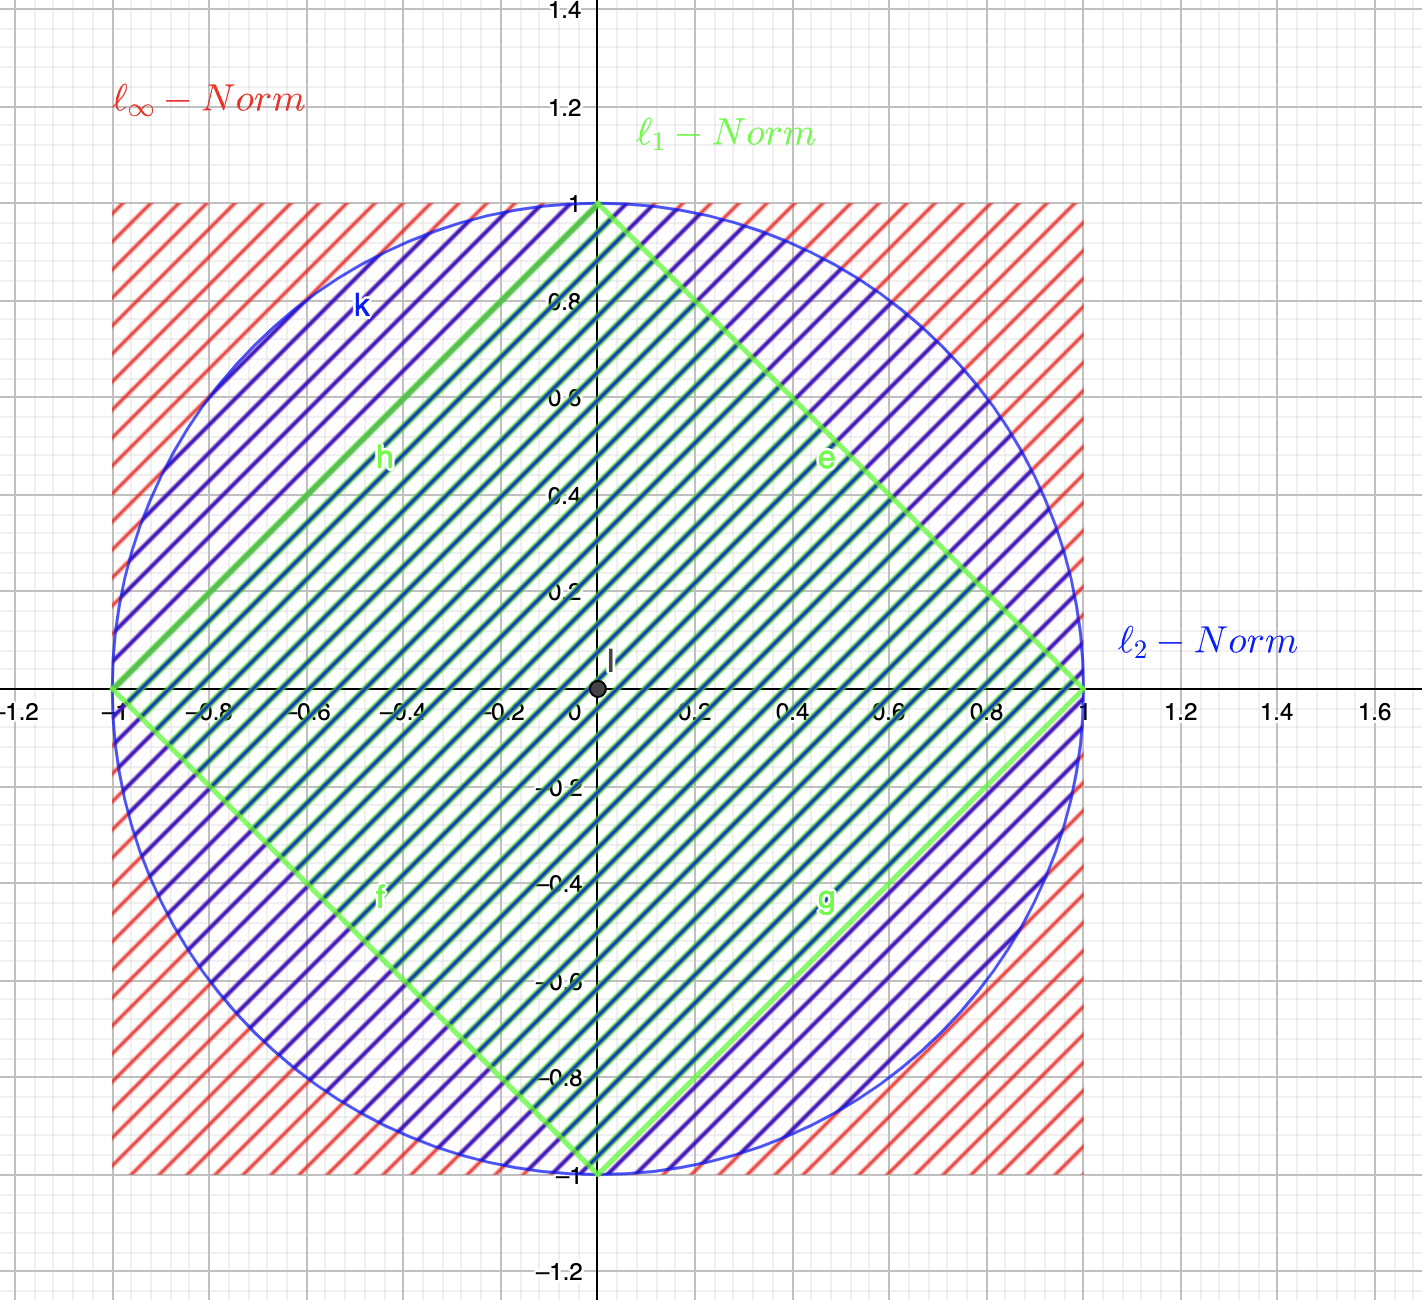
\includegraphics[width=\linewidth]{Bilder/Norms}
	\label{normbild}
\end{figure}\par
\end{titleDef}

\begin{titleDef}{Metrik}
\label{Metrik}
Sei X eine Menge. Eine Abbildung $d:X\times X:\to \mathbb{R}_{\ge0}$ ist eine \textbf{Metrik}, falls für alle $x,y,c\in X$ gilt:
\begin{enumerate}
    \item positiv definit: $d(x,y)=0\Leftrightarrow x=y$
    \item symmetrisch: $d(x,y)=d(y,x)$
    \item Dreickesungleichung: $d(x,z)\le d(x,y)+d(y,z)$
\end{enumerate}
\end{titleDef}

\begin{titleDef}{Abstandserhaltend}
\label{abstandserhaltend}
Seien $(X,d_X),(Y,d_Y)$ \hyperref[MetrischerRaum]{metrische Räume}. Eine Abbildung $f:X\to Y$ heißt abstandserhaltend, falls für alle $x,y\in X$ gilt: $d_Y(f(x),f(y))=d_X(x,y)$
\end{titleDef}

\begin{titleDef}{Isometrie}
\label{Isometrie}
Eine Isometrie ist eine bijektive, \hyperref[abstandserhaltende]{abstandserhaltend} Abbildung.\par
Seien $S,\tilde{S}$ \hyperref[regFlaeche]{reguläre Flächen}. Eine Abbildung $f:S\to\tilde{S}$ heißt \textbf{Isometrie}, wenn $f$ ein \hyperref[diffeomorph]{Diffeomorphismus} zwischen $S$ und $\tilde{S}$ ist und für alle \hyperref[diffFlaechenkurve]{differenzierbaren Kurven} $c:I\to S$ gilt, dass die \hyperref[laengeFlaechenkurve]{Länge der Kurve} unter $f$ invariant ist also $L(f\circ c)=L(c)$.\\
Für die metrischen Räume auf den regulären Flächen $(S,d_S),(\tilde{S},d_{\tilde{S}})$ gilt insbesondere $d_{\tilde{S}}(f(p),f(q))=d_S(p,q)$
\end{titleDef}

\begin{titleDef}{lokale Isometrie}
\label{lokIso}
Eine Abbbildung $f:S\to\tilde{S}$ zwischen \hyperref[regFlaeche]{regulären Flächen} $S,\tilde{S}$ heißt \textbf{lokale Isometrie}, falls für jeden Punkt $p\in S$ eine \offUm $U\subset S$ von p und $V\subset\tilde{S}$ von $f(p)$ existiert, so dass $f$ eingeschränkt auf $U$ eine Isometrie zwischen $U$ und $V$ ist.\par
Sind $S,\tilde{S}$ \hyperref[regFlaeche]{reguläre Flächen} mit \hyperref[parametrisierung]{Parametrisierungen}
$$x:U\to x(U)\subset S\qquad \tilde{x}:U\to \tilde{x}(U)\subset\tilde{S}$$
so dass die \hyperref[fundamentalformEins]{1.Fundamentalform} von $S$ und $\tilde{S}$ in den Punkten $(u,v)\in U$ aus $U$ übereinstimmen, also
$$
	\begin{pmatrix} 
	\mathrm{E}(u,v) & \mathrm{F}(u,v)\\
	\mathrm{F}(u,v) & \mathrm{G}(u,v)
\end{pmatrix} = 
	\begin{pmatrix} 
	\mathrm{\tilde{E}}(u,v) & \mathrm{\tilde{F}}(u,v)\\
	\mathrm{\tilde{F}}(u,v) & \mathrm{\tilde{g}}(u,v)
\end{pmatrix} 
$$
Dann sind $x(U)\subset S$ und $\tilde{x}(U)\subset\tilde{S}$ isometrisch.
\end{titleDef}

\begin{titleDef}{Stetigkeit}
\label{stetig}
Seien $(X,\mathcal{O}_X)$ und $(Y,\mathcal{O}_Y)$ \hyperref[Topologie]{topologische Räume}.\\
Eine Abbildung $f:X\to Y$ heißt \textbf{stetig}, falls die Urbilder von offenen Mengen in Y stets offen sind in X.
$$\text{f stetig} \Leftrightarrow \text{Für alle } V\in\mathcal{O}_Y \text{ ist } f^{-1}=\{x\in X|\ f(x)\in V\}\in\mathcal{O}_X$$\\
Folgende Aussagen sind äquivalent:
\renewcommand{\labelenumi}{(\roman{enumi})}
\begin{enumerate}
    \item f ist stetig
    \item Für alle $x\in X$ gilt:
    $$\forall\varepsilon>0\ \exists \delta=\delta(\varepsilon,x), \text{ so dass } f(B_\delta^X(x))\subseteq B_\varepsilon^Y(f(x))$$
    \item f ist folgenstetig, d.h für alle $x\in X$ gilt
    $$x=\lim_{x\to\infty}x_n \Rightarrow f(x)=\lim_{n\to\infty}f(x_n)$$
\end{enumerate}
Jede stetige Funktion auf einer \hyperref[kompakt]{kompakten Teilmenge} eines \hyperref[Topologie]{topologischen Raumes} hat ein endliches Maximum und Minimum, ist also insbesondere beschränkt.
\end{titleDef}

\begin{titleDef}{Homöomorphismus}
\label{homoemorph}
Eine bijektive Abbildung zwischen \hyperref[Topologie]{topologischen Räumen} $f:X\to Y$ heißt \textbf{Homöomorphismus}, falls $f$ und ihre Umkehrabbildung $f^{-1}$ stetig sind, d.h:
\begin{align*}
    \text{f ist homöomorphismus}&\Longleftrightarrow f\text{ bijektiv und }f,f^{-1}\text{ stetig}\\
    &\Longleftrightarrow U\subseteq X\text{offen}\Longleftrightarrow f(U)\subseteq Y\text{offen}
\end{align*}\\
Damit ist homöomorphismus stärker als stetigkeit weil bei Stetigkeit nur $$f^{-1}(U)\subseteq Y\text{ offen}\Rightarrow U\subseteq X\text{ offen gilt.}$$
Die \hyperref[Topologie]{topologischen Räumen} $X$ und $Y$ heißen \textbf{homöomorph} wenn es einen Homöomorphismus $f:X\to Y$ gibt. Geschrieben $X\simeq Y$.\\
\textbf{Beispiel:}
\listbsp
\begin{enumerate}
    \item Alle abgeschlossenen Intervalle bzgl der \hyperref[stdTopo]{Standard-Topologie} sind homöomorph:
    $$[0,1]\simeq [a,b]\text{ für alle }a<b\in\mathbb{R}$$
    Gleiches gilt für die offenen intervalle $(0,1)\simeq (a,b)$. Ein Homöomorphismus ist gegeben durch $f(t)=a+t(b-a)$
    \item Ganz $\mathbb{R}$ ist bzgl der \hyperref[stdTopo]{Standard-Topologie} homöomorph zu einem offenen Intervall:
    $$\mathbb{R}\simeq(-1,1)\simeq(0,1)$$
    Ein Homöomorphismus ist gegeben durch $f(t)=tanh(t)=\frac{e^{2t}-1}{e^{2t}+1}$
    \item Seien $(X,d_X),(Y,d_Y)$ \hyperref[MetrischerRaum]{metrische Räume} und $f:X\to Y$ eine \hyperref[Isometrie]{Isometrie}. Dann ist $f$ ein Homöomorphismus. Setzte $\varepsilon=\delta$ dann:
    $$d_X(x,y)<\delta \Rightarrow d_Y(f(x),f(y))=d_X(x,y)<\delta=\varepsilon$$
    Also wenn ein Punkt x im \hyperref[balloffen]{Delta-Ball} $B_{\delta}(y)$ um y liegt, dann liegt f(x) im \hyperref[balloffen]{Epsilon-Ball} $B_{\varepsilon}(f(y))$ um f(y) für beliebige x und y. Also $f(B_{\delta}(y))\subseteq B_{\varepsilon}(f(y))$ und damit sind die Bilder von offenen Mengen unter f wieder offen und analog umgekehrt.
    \item \begin{titleDef}{stereographische Projektion}
    \label{stereoproj}
    Sei $S^n=S^n_1=\{x\in\mathbb{R}^{n+1}|\ \lVert x\rVert^2=x_1^2+\dots+x_{n+1}^2=1\}$ die \hyperref[ndimsphere]{n-dimensionale Sphäre vom Radius 1}. Weiter sei $e_{n+1}=(0,\ldots,0,1)\in S^{n+1}$ der \hyperref[pol]{Nordpol}. Dann ist $S^n$ homöomorph zu $\mathbb{R}^n:S^n\textbackslash\{e_{n+1}\}\simeq\mathbb{R}^n$. Ein Homöomorphismus ist die \textbf{stereographische Projektion}
    $$spr:S^n\textbackslash\{e_{n+1}\}\to\mathbb{R}^n;\ spr(x)=\left(\frac{x_1}{1-x_{n+1}},\cdots,\frac{x_n}{1-x_{n+1}}\right)$$
    Für die Umkehrabbildung gilt:
    $$spr^{-1}:\mathbb{R}^n\to S^n\textbackslash\{e_{n+1}\};\ spr^{-1}(y)=\left(\frac{2y_1}{\lVert y\rVert^2+1},\cdots,\frac{2y_n}{\lVert y\rVert^2+1}, \frac{\lVert y\rVert^2-1}{\lVert y\rVert^2+1}\right)$$
    \end{titleDef}
\end{enumerate}
Eine \hyperref[stetig]{stetige},bijektive Abbildung $f:X\to Y$ von einem \hyperref[kompakt]{kompakten Raum} $X$ auf einen \hyperref[hausdorffsch]{hausdorffschen Raum} $Y$ ist ein Homöomorphismus.
\end{titleDef}

\begin{titleDef}{Reguläre Kurve}
\label{kurve}
Eine (reguläre) \textbf{Kurve} ist eine differenzierbare Abbildung $c:[a,b]\to\mathbb{R}^n;t\mapsto c(t)$, so dass $c^\prime(t)=\frac{dc}{dt}\neq 0$.
\end{titleDef}

\begin{titleDef}{differenzierbare Flächenkurve}
\label{diffFlaechenkurve}
Eine differenzierbare Flächenkurve ist differenzierbare Abbildung auf einer \hyperref[regFlaeche]{regulären Fläche} mit Parametrisierung $x(u,v)$
$$c:[\alpha,\beta]\to S;\: t\mapsto x(u(t),v(t))$$
\end{titleDef}

\begin{titleDef}{Tangentialvektor}
\label{tangentialvektor}
Sei S eine \hyperref[regFlaeche]{reguläre Fläche} mit Parametrisierung $x(u,v)$ und $c$ eine \hyperref[diffFlaechenkurve]{differenzierbare Flächenkurve}. Der \textbf{Tangentialvektor} an $c$ im Punkt $c(t)\in S$ ist gegeben durch:
$$c^\prime(t)=x_u(u(t),v(t))u^\prime(t)+x_v(u(t),v(t))v^\prime(t)\in T_{c(t)}S$$
\end{titleDef}

\begin{titleDef}{Länge von Flächenkurven}
\label{laengeFlaechenkurve}
Sei S eine \hyperref[regFlaeche]{reguläre Fläche} mit Parametrisierung $x(u,v)$ und $c$ eine \hyperref[diffFlaechenkurve]{differenzierbare Flächenkurve}. Die \textbf{Länge} der Kurve $c$ ist gegeben durch:
$$L(c)=\int_{\alpha}^{\beta}\lVert c^\prime(t)\rVert_{c(t)}dt$$
\end{titleDef}

\begin{titleDef}{Winkel zwischen Flächenkurven}
\label{winkelFlaechenkurve}
Sei S eine \hyperref[regFlaeche]{reguläre Fläche} und $c_1,c_2$ \hyperref[diffFlaechenkurve]{differenzierbare Flächenkurven}. Der Winkel zwischen diesen beiden Kurve ist gegeben durch:

$$\cos\angle(c^\prime_1(0),c^\prime_2(0))=
\frac{\langle c_1^\prime(0),c_2^\prime(0)}{\lVert c_1^\prime(0)\rVert\lVert c_2^\prime\rVert}$$
\end{titleDef}

\begin{titleDef}{Flächeninhalt Parametrisierung}
\label{inhaltPara}
Sei S eine \hyperref[regFlaeche]{reguläre Fläche} mit Parametrisierung $x:U\to x(U)\subset S\subset\Rthree$. Dann ist der \textbf{Flächeninhalt} der Parametrisierung $x(U)$ definiert als:
$$A(x(U))=\int\int_{U}\lVert x_u\wedge x_v\rVert dudv=
\int\int_{U}\sqrt{EG-F^2} dudv=\int\int_{U}det(I) dudv$$
\end{titleDef}

\begin{titleDef}{Differenzierbar}
\label{differenzierbar}
Seien $M$ und $N$ \hyperref[diffMannigfaltigkeit]{differenzierbare Mannigfaltigkeiten} mit \hyperref[dimMannigfaltigkeit]{Dimensionen} dim$(M) = m$ und dim$(N)=n$. Eine \hyperref[stetig]{stetige} Abbildung $f:M\to N$ heißt \textbf{differenzierbar in }$p\in M$, falls für \hyperref[Karte]{Karten} $(U,\varphi)$ um den Punkt $p\in M$ und $(V,\psi)$ um den Bildpunkt $f(p)\in N$, wenn die Koordinatendarstellung $\psi\circ f\circ\varphi^{-1}$ von $f$ bei $p$ im Punkt $\varphi(p)\: C^\infty$ ist.
$$\psi\circ f\circ\varphi^{-1}:\varphi(U)\subset\mathbb{R}^m\to\psi(V)\subset\mathbb{R}^n$$
Analog heißt $f$ \textbf{differenzierbar} wenn $f$ in jedem Punkt $p\in M$ differenzierbar ist.
\end{titleDef}

\begin{titleDef}{Differential}
\label{differenzial}
Für eine \hyperref[differenzierbar]{differenzierbare} Abbildung $f:\mathbb{R}^m\to\mathbb{R}^n$ ist die \textbf{Ableitung bzw das Differential} von $f$ in $p\in\mathbb{R}^m$ definiert als lineare Abbildung\\ ${df(p):T_p\mathbb{R}^m\cong\mathbb{R}^m\to T_{f(p)}\mathbb{R}^n\cong\mathbb{R}^n}$
die $f$ in einer \hyperref[Umgebung]{Umgebung} von $p$ approximiert.
\end{titleDef}

\begin{titleDef}{kovariante Ableitung}
\label{kovAbleitung}
\label{tangentialesVektorfeld}
Sei $S$ eine \hyperref[regFlaeche]{reguläre Fläche} mit Parametrisierung $x:U\to S$. Weiter sei $a:U\to\Rthree$ ein \hyperref[vektorenfeld]{tangentiales Vektorenfeld} längs $S$, d.h für alle $(u,v)\in U$ liegt $a(u,v)\in T_{x(u,v)}S$ in der \hyperref[tangentialebene]{Tangentialebene} $T_{x(u,v)}S$ und insbesondere ist $a(u,v)$ orthogonal zum \hyperref[normalenvektor]{Normalenvektor} $n(u,v)$.\\
Weil $a_u(u,v)=\frac{\partial}{\partial u}a(u,v)\in T_{x(u,v)}\Rthree$ im Allgemeinen nicht mehr in $T_{x(u,v)}S$ definiert man die \textbf{kovariante Ableitung} $D_ua$ von $a$ nach $u$ als die Orthogonalprojektion von $a_u$ in die \hyperref[tangentialebene]{Tangentialebene}
$$D_ua=a_u-\langle n,a_u\rangle n=a_u+\langle n_u,a\rangle n$$
\end{titleDef}

\begin{titleDef}{Diffeomorphismus}
\label{diffeomorph}
Ein \textbf{Diffeomorphismus} ist eine bijektive Abbildung $f:M\to N$ zwischen \hyperref[diffMannigfaltigkeit]{differenzierbaren Mannigfaltigkeiten } $M,N$, die sowohl selbst als auch ihre Umkehrabbildung $f^{-1}:M\to N$ differenzierbar ist.\\
Ein Diffeomorphismus ist immer auch ein \hyperref[homoemorph]{Homöomorphismus}. 
\end{titleDef}

\begin{titleDef}{Triangulierung}
\label{triangulierung}
Sei $M$ eine \hyperref[kompakt]{kompakte}~\hyperref[orientierbar]{orientierbare} \hyperref[Mannigfaltigkeit]{2-Mannigfaltigkeit}. Eine \textbf{Triangulierung} $T$ von $M$ ist eine endliche Famillie von (orientierungserhaltenden) \hyperref[diffeomorph]{Diffeomorphismen}
$$\delta_k:\Delta\to\delta_k(\Delta)\subset M$$
des \hyperref[stdSimplex]{Standard-2-Simplex} $\Delta$ (also eines Dreiecks) nach $M$ sodass gilt:
\begin{enumerate}[label=(\arabic*)]
	\item Die Bild-Simplizes (Dreiecke) $\delta_k(\Delta)$ überdecken $M$: $M=\bigcup_{k=1}^n\delta_k(\Delta)$
	\item Ist $\delta_k(\Delta)\cap\delta_j(\Delta)\neq\emptyset$ für $k\neq j$ so haben $\delta_k(\Delta)$ und $\delta_j(\Delta)$ entweder genau eine gemeinsame Ecke oder genau eine gemeinsame Kante nur eines von beiden und nicht mehr.
\end{enumerate}\par
Jede \hyperref[kompakt]{kompakte}, \hyperref[orientierbar]{orientierbare} 2-Mannigfaltigkeit $M$ mit Atlas $\mathcal{A}$ besitzt eine \hyperref[triangulierung]{Triangulierung} $\delta_k:\Delta\to\delta_k(\Delta)\subset M$, so dass jedes \hyperref[simplex]{Simplex} $\delta_k(\Delta)$ ganz in einer Kartenumgebung von $\mathcal{A}$ enthalten ist.
\end{titleDef}





\clearpage
\section{Geometrische Strukturen}
\begin{titleDef}{Metrische Räume}
\label{MetrischerRaum}
Ein Paar (X,d) aus einer Menge X und einer \hyperref[Metrik]{Metrik} heißt metrischer Raum.\\
Metrische Räume sind \hyperref[hausdorffsch]{hausdorffsch}.
\end{titleDef}

\begin{titleDef}{Topologische Räume}
\label{Topologie}
Ein topologischer Raum ist ein Paar $(X,\mathcal{O})$ bestehend aus einer Menge X und einem System $\mathcal{O}\subseteq\mathcal{P}(X)$ von Teilmengen von X, so dass gilt
\begin{enumerate}
    \item $X,\emptyset\in\mathcal{O}$
    \item Der Durchschnitt von endlich vielen Mengen aus $\mathcal{O}$ ist wieder in $\mathcal{O}$$$\Leftrightarrow\bigcap^n_{i=1}X_i\in\mathcal{O}, n\in\mathbb{N},X_i\in\mathcal{O}$$
    \item Die Vereinigung von beliebig vielen Mengen aus $\mathcal{O}$ ist wieder in $\mathcal{O}$\\$$\Leftrightarrow\bigcup_{i=1}^kX_i\in\mathcal{O}, k\in\mathbb{N}\cup\{\infty\},X_i\in\mathcal{O}$$
\end{enumerate}
Ein solches System $\mathcal{O}$ von Teilmengen heißt \textbf{Topologie} von X 
\end{titleDef}

\begin{titleDef}{Umgebung}
\label{Umgebung}
Sei $B\subset X$ eine Teilmenge von X einer \Toporef \Topo. Eine Teilmenge ${U\subseteq X}$ heißt Umgebung von B, falls eine offene Menge O bezüglich der \Toporef existiert, so dass $B\subseteq O\subseteq U$. Also B ist komplett in einer offenen Teilmenge von X enthalten. Beachte das B nicht offen sein muss.
\end{titleDef}

\begin{titleDef}{Topologische Mannigfaltigkeiten}
\label{Mannigfaltigkeit}
Eine \textbf{(topologische) Mannigfaltigkeit} ist ein \Toporeflong $M$ mit:
\listbsp
\begin{enumerate}
	\item $M$ ist \textbf{lokal euklidisch}, d.h für alle Punkte $p\in M$ existiert eine \hyperref[offen]{offene} \hyperref[Umgebung]{Umgebung} $U$ von $p$ und ein \hyperref[homoemorph]{Homöomorphismus} ${\varphi:U\to \varphi(U)\subseteq\mathbb{R}^n}$ auf eine offene Teilmenge von $\mathbb{R}^n$ für gewisses n.
	\item $M$ ist \hyperref[hausdorffsch]{Hausdorffsch} und hat eine abzählbare \hyperref[basisTopo]{Basis}.
\end{enumerate}
\end{titleDef}

\begin{titleDef}{Differenzierbare Mannigfaltigkeit}
\label{diffMannigfaltigkeit}
Eine \textbf{Differenzierbare Mannigfaltigkeit} ist eine topologische Mannigfaltigkeit versehen mit einem \hyperref[maxAtlas]{maximalen Atlas}.
\end{titleDef}

\begin{titleDef}{Simplizialkomplexe}
\label{simplex}
Ein \textbf{k-Simplex} in $\mathbb{R}^n$ ist die \hyperref[konvHuelle]{konvexe Hülle} $s(v_0,v_1,\ldots,v_k)$ von k+1 affin unabhängigen Punkten $v_0,v_1,\ldots,v_k$.\par
Eine endliche Menge $K$ von Simplexen heißt (endlicher) $\textbf{Simplizial-Komplex}$ wenn gilt:
\begin{enumerate}
	\item Mit jedem Simplex in K enthält K auch alle zugehörigen Teilsimplexe.\\Also wenn das "Dreieck" $s(v_0,v_1,v_2)\in K$ dann gilt: Die Seiten $s(v_0,v_1)\in K,s(v_0,v_2)\in K,s(v_1,v_2)\in K$ sowie die Punkte $s(v_0)\in K,s(v_1)\in K,s(v_2)\in K$ liegen in K.
	\item Der Durchschnitt von zwei Simplexen die in K liegen ist entweder leer oder \textbf{genau} ein gemeinsames Teilsimplex.\\
	Also schneiden sich zwei Simplexe entweder gar nicht, in genau einem Punkt oder genau einer vollständigen Seite, usw
\end{enumerate}
Simplizialkomplexe entstehen durch \hyperref[verklebung]{verkleben} von Simplexen.
\end{titleDef}

\begin{titleDef}{konvexe Polyeder}
\label{konvexPoly}
Eine Teilmenge $P\subset\mathbb{R}^3$ heißt \textbf{konvexes Polyeder}, falls
\begin{enumerate}
	\item $P$ ist Durchschnitt von endlich vielen affinen Halbräumen\\
	Ein affiner Halbraum kann man sich als die linke oder rechte Hälfte einer Ebene durch den $\mathbb{R}^3$ vorstellen.
	\item $P$ ist beschränkt und nicht ganz in einer Ebene enthalten.
	\item $P$ ist konvex, d.h. mit je zwei Punkten $p,q\in P$ liegt auch das Geradensegment $\overline{pq}$ ganz in $P$.
\end{enumerate}
Eigenschaft 3. ist nicht notwendig für einen konvexen Polyeder gilt aber wenn eine Teilmenge ein konvexes Polyeder ist.\par
Ein Polyeder heißt (m,n)-\textbf{regulär}, falls alle Seitenflächen des Polyeders n-Gone sind also alle Kanten gleich lang sind und in jeder Ecke genau m solcher n-Gone /Kanten zusammentreffen.
\end{titleDef}

\begin{titleDef}{Reguläre Flächen}
\label{regFlaeche}
Eine Teilmenge $S\subset\mathbb{R}^3$ heißt \textbf{reguläre Fläche}, falls es zu jedem Punkt $p\in S$ eine \hyperref[offen]{offene} \hyperref[Umgebung]{Umgebung} $V$ um $p$ in $\mathbb{R}^3$, eine \hyperref[offen]{offene} \hyperref[Umgebung]{Umgebung} $U\subset\mathbb{R}^2$ und eine $C^\infty$-Abbildung die sogenannte \textbf{(lokale) Parametrisierung}
$$x:U\to\mathbb{R}^3;\: (u,v)\mapsto x(u,v)=(x_1(u,v),x_2(u,v),x_3(u,v))$$
gibt, so dass
\begin{enumerate}[label=(\arabic*)]
	\item $x(U)=S\cap V$ und $x:U\to S\cap V$ ist ein \hyperref[homoemorph]{Homöomorphismus} 
	\item Die \hyperref[differenzial]{Ableitung} $dx(u,v):T_{(u,v)}\mathbb{R}^2\to T_{x(u,v)}\mathbb{R}^3$ ist injektiv für $(u,v)\in U$
\end{enumerate}
Bedingung (2) ist äquivalent zu
\begin{enumerate}[label=(2\alph*)]
	\item Die \hyperref[funktmatrix]{Funktionalmatrix} $\begin{pmatrix}
		\frac{\partial x_1}{\partial u}(u,v)&\frac{\partial x_1}{\partial v}(u,v)\\
		\frac{\partial x_2}{\partial u}(u,v)&\frac{\partial x_2}{\partial v}(u,v)\\
		\frac{\partial x_3}{\partial u}(u,v)&\frac{\partial x_3}{\partial v}(u,v)\\
		\end{pmatrix}$ hat Rang 2 für $(u,v)\in U$
	\item Die Spaltenvektoren $x_u(u,v),\ x_v(u,v)$ sind linear unabhängig.
	\item Das \hyperref[vektorprodukt]{Vektorprodukt} $x_u(u,v)\wedge x_v(u,v)\neq0$ für alle $(u,v)\in U$
\end{enumerate}
\end{titleDef}

\begin{titleDef}{Polygon}
\label{polygon}
\label{innenwinkel}
Sei $S$ eine \hyperref[regFlaeche]{reguläre Fläche}. Ein \textbf{Polygon} in $S$ ist eine Teilmenge $G$, die \hyperref[homoemorph]{homöomorph} zu einer \hyperref[abgeschlossen]{abgeschlossenen} Kreisscheibe ist und deren Rand $\partial G$ das Bild einer \hyperref[einfachgeschlossen]{einfach geschlossenen}, stückweise \hyperref[regulaer]{regulären} Kurve ist. Die \textbf{Innenwinkel} des Polygons sind durch $\alpha_i=\pi-\delta_i$ mit den \hyperref[aussenwinkel]{Außenwinkeln} $\delta_i$
\end{titleDef}

\begin{titleDef}{geodätische Dreiecke}
\label{geodaetischeDreiecke}
Ein \textbf{geodätisches Dreieck} in einer \hyperref[regFlaeche]{regulären Fläche} S ist ein \hyperref[polygon]{Polygon} $\Delta$, das genau drei Ecken hat und dessen drei Randsegmente/Kanten \hyperref[geodaetische]{Geodätische} sind.\par
Seien $\alpha,\beta,\gamma$ die Innenwinkel des geodätischen Dreiecks. Für die Innenwinkelsumme eines geodätischen Dreiecks in einer Fläche $S$ die konstante \hyperref[gausskruemmung]{Gaußkrümmung K} haben gilt:
\begin{itemize}
	\item Für $K\equiv0\Longrightarrow \alpha+\beta+\gamma=\pi$
	\item Für $K\equiv1\Longrightarrow \alpha+\beta+\gamma>\pi$
	\item Für $K\equiv-1\Longrightarrow \alpha+\beta+\gamma<\pi$
\end{itemize}
\end{titleDef}



\clearpage
\section{Topologien}
\begin{titleDef}{Triviale Topologie}
\label{trivTopo}
Die kleinstmögliche Topologie $(X,\mathcal{O}_t)$ mit $\mathcal{O}_t=\{X,\emptyset\}$ heißt \mbox{\textbf{triviale Topologie}} auf $X$
\end{titleDef}

\begin{titleDef}{Diskrete Topologie}
\label{diskTopo}
Die größtmögliche Topologie $(X,\mathcal{O}_d)$ mit $\mathcal{O}_d=\mathcal{P}(X)$ heißt \mbox{\textbf{diskrete Topologie}} auf $X$
\end{titleDef}

\begin{titleDef}{Standard Topologie}
\label{stdTopo}
Sei $X=\mathbb{R}$ die Menge der reellen Zahlen und\\ ${\mathcal{O}_s=\{I\subseteq\mathbb{R}| \ I=\text{Vereinigung von offenen Interevallen} (a,b),a,b\in\mathbb{R}\}}$\\
dann heißt $(X,\mathcal{O}_s)$ die \mbox{\textbf{Standardtopologie}} auf $\mathbb{R}$.
Die Standardtopologie hat eine abzählbare Basis.\\
Die Standardtopologie bezüglich den reellen Zahlen $(\mathbb{R},\mathcal{O}_s)$ ist \hyperref[hausdorffsch]{hausdorffsch}\\
Die reellen Zahlen $\mathbb{R}$~mit der Standard-Topologie und auch alle Intervalle $I\subset\mathbb{R}$~sind \hyperref[zusammenhang]{zusammenhängend}
\end{titleDef}

\begin{titleDef}{Metrisch induzierte Topologie}
\label{metTopo}
\hyperref[MetrischerRaum]{Metrische Räume} (X,d) sind topologische Räume, also wird durch eine \hyperref[Metrik]{Metrik} eine Topolgie induziert, die aus den \hyperref[doffen]{d-offenen} Mengen von X besteht.
\\Die Topologie induziert von der \hyperref[stdmetrik]{Standard Metrik} hat eine abzählbare Basis bestehend aus allen rationalen \hyperref[balloffen]{Bällen} mit rationalen Radien und rationalen Zentren.
\end{titleDef}

\begin{titleDef}{Basis}
\label{basisTopo}
Sei \Topo ein \Toporef. Eine \textbf{Basis} für die Topologie $\mathcal{O}$ ist eine Teilmenge $\mathcal{B}\subseteq\mathcal{O}$ so dass für jede offene Menge $V\neq\emptyset, V\in\mathcal{O}$ gilt:
$$V=\bigcup_{i\in I}V_i, \ V_i\in\mathcal{B}$$
\end{titleDef}

\begin{titleDef}{Teilraumtopologie}
\label{teilraumTopo}
Sei $(X,\mathcal{O}_X)$ ein topologischer Raum und $Y\subset X$ eine Teilmenge von X. Die \mbox{\textbf{Teilraumtopologie}} von Y ist gegeben durch 
$$\mathcal{O}_Y=\{U\subseteq Y|\ U\cap Y \text{ für ein }V\in\mathcal{O}_X\}$$
und macht damit $(X,\mathcal{O}_Y)$ zu einem topolgischen Raum bezüglich dieser Teilraumtopologie
\end{titleDef}

\begin{titleDef}{Produkttopologie}
\label{produktTopo}
Seien $(X,\mathcal{O}_X),\ (Y,\mathcal{O}_Y)$ zwei topolgische Räume. Eine Teilmenge $W\subseteq X\times Y$ ist offen in der \mbox{\textbf{Produkt-Topologie}} wenn es zu jedem Punkt $(x,y)\in W$ eine \hyperref[Umgebung]{Umgebung} $U\subseteq X$ von x und eine \hyperref[Umgebung]{Umgebung} $V\subseteq Y$ von y gibt, so dass $U\times V\subseteq W$ gilt.\\
Also man findet um jeden Punkt einer offenen Menge koordinatenweise offene Mengen bezüglich der komponententopologien die vollständig in einer Umgebung der entsprechenden Menge liegt.
\end{titleDef}

\begin{titleDef}{Quotiententopologie}
\label{quotTopo}
Sei $(X,\mathcal{O}_X)$ ein topologischer Raum und $\sim$ eine Äquivalenzrelation auf der Menge $X$. Die Äquivalenzklasse eines Elementes $x\in X$ ist gegeben durch $[x]=\{y\in X|\ x\sim y\}$.Die Äquivalenzklassen bilden eine Partition von $X$ sind also eine disjunkte Zerlegung dessen Vereinigung wieder den Gesamtraum ergibt. $X/\sim$ ist dann der zugehörige Qutienten-Raum auf dem die \textbf{Quotiententopologie} definiert ist.
$$\pi:X\to X/\sim;\ x\mapsto[x]$$
ist die kanonische Projektion die Elemente auf ihre Äquivalenzklasse abbildet. $\pi$ ist eine \hyperref[stetig]{stetige Funktion} (insbesondere ist damit auch $\pi\times\pi:X\times X\to Y\times Y)$ usw. stetig in der Produkttopologie wobei $\pi^{-1}(U,V)=\pi^{-1}(U)\times \pi^{-1}(V)$).\\
Die \textbf{Quotiententopologie} $(X/\sim,\mathcal{O}_{X/\sim})$ ist dann definiert durch die offenen Mengen:
$$U\subseteq X/\sim offen \Longleftrightarrow \pi^{-1}(U)=\{x\in X|\ \pi(x)=[x]\in U\} offen in X$$
Also eine Menge $U$ ist offen bezüglich der Quotiententopologie, wenn die Menge der Urbilder der Äquivalenzklassen die in der $U$ liegen eine offene Menge bezüglich der Topologie auf $X$ bilden.
\end{titleDef}


\begin{titleDef}{Projektiver Raum $P^n$}
	\label{projRaum}
	Der projektive Raum ist eine abstrakte \hyperref[Mannigfaltigkeit]{Mannigfaltigkeit} deren Elemente gerade die Geraden in $\mathbb{R}^{n+1}$ durch den Nullpunkt sind. Definiere also den projektiven Raum $P^n=\{\text{eindimensionale Unterräume von }\mathbb{R}^{n+1}\}$.\par
	Um $P^n$ zu einem topologischen Raum zu machen gibt es zwei Betrachtungsmöglichkeiten:
	\begin{enumerate}[label=(\alph*)]
		\item Definiere auf $\mathbb{R}^{n+1}\setminus\{0\}$ die Äquivalenzrelation
		$$x\sim y\Longleftrightarrow\ \exists\lambda\neq0 \text{ mit }x= \lambda y$$
		Dann ist $P^n=\mathbb{R}^{n+1}\setminus\{0\}/\sim$
		\item Definiere auf der \hyperref[ndimsphere]{n-Sphäre} $S_1^n=S^n$ die Äquivalenzrelation ${x\sim y\Longleftrightarrow x=-y}$. Eine Äquivalenzklasse ist also gegeben durch $[x]=\{x,-x\}$ und $P^n=S^n/\sim$
	\end{enumerate}
Damit kann als \hyperref[Topologie]{Topologie} von $P^n$ die \hyperref[quotTopo]{Quotienten-Topologie} von $S^n/\sim$ definieren.\\
$P^n$ ist eine \hyperref[kompakt]{kompakte} \hyperref[diffMannigfaltigkeit]{n-dimensionale differenzierbare Mannigfaltigkeit}.\\
Insbesondere ist $P^n$ \hyperref[hausdorffsch]{hausdorffsch} und hat eine \hyperref[basisTopo]{abzählbare Basis}\par
Ein Atlas $\mathcal{A}=\{(U_i,\varphi_i)|\: i=1,\ldots,n+1\}$ ist gegeben durch:
$$U_i=\{[(x_1,\ldots,x_{n+1})]\in P^n|\ x_i\neq0\}$$
$$\varphi_i:U_i\to\mathbb{R}^n;\:\:[(x_1,\ldots,x_{n+1})]\mapsto\varphi_i([(x_1,\ldots,x_{n+1})])=\frac{1}{x_i}(x_1,\ldots,x_{i-1},x_{i+1},\ldots,x_{n+1})$$
Die Umkehrabbildung ist einfach gegeben durch:
$$\varphi_i^{-1}:\mathbb{R}^n\to U_i\:\:\:(x_1,\ldots,x_n)\mapsto[(x_1,\ldots,x_{i-1},1,x_{i+1},\ldots,x_{n+1})]$$
und natürlich ist auch $\varphi_i^{-1}$ stetig (muss es ja sein damit wir eine diffbare Mannigfaltigkeit bekommen)
\end{titleDef}

\begin{titleDef}{Simplizial topologischer Raum}
\label{simplexTopo}
Ein \hyperref[simplex]{Simplizialkomplex} $K$ kann zu einem topologischen Raum erweitert werden. Die Menge $\lvert K\rvert=\bigcup_{s\in K}s\subset\mathbb{R}^n$ versehen mit der \hyperref[teilraumTopo]{Teilraum-Topologie} von $\mathbb{R}^n$ heißt der zum Simplizialkomplex $K$ gehörende topologische Raum.
\end{titleDef}

\begin{titleDef}{Klassifikation 2-dimensionaler Mannigfaltigkeiten/Geschlecht}
\label{geschlecht}
Sei $M$ eine \hyperref[kompakt]{kompakte} \hyperref[orientierbar]{orientierbare} 2-dimensionale topologische Mannigfaltigkeit. Dann gibt es eine natürliche Zahl $\mathbb{N}\ni g\geq 0$ das sogenannte \textbf{Geschlecht}. Es gilt:
\begin{itemize}
	\item Die Sphäre $S^2_R$ hat Geschlecht 0
	\item Der Torus hat Geschlecht 1
	\item Falls $g=0$ so ist $M$ \hyperref[homoemorph]{homöomorph} zur \hyperref[sphere]{Sphäre} $S^2=S^2_1$
	\item Falls $g\geq1$ so ist $M$ \hyperref[homoemorph]{homöomorph} zu einer \hyperref[zusammenhang]{zusammenhängenden} Summe von $g$ \hyperref[torus]{Tori}.
	\item Zwei \hyperref[kompakt]{kompakte} \hyperref[orientierbar]{orientierbare} Flächen/Mannigfaltigkeiten mit gleichen Geschlecht immer homöomorph
\end{itemize}
\end{titleDef}

\clearpage
\section{Mannigfaltigkeiten}
\begin{titleDef}{Karte}
\label{Karte}
Eine \textbf{Karte} ist ein Paar $(U,\varphi)$ mit Eigenschaft (1) einer \hyperref[Mannigfaltigkeit]{(topologischen) Mannigfaltigkeit $M$}. Der \Toporeflong~Raum $M$ ist also \hyperref[lokaleukldisch]{lokal euklidisch} d.h $U$ ist offene Umgebung um eine Menge von Punkten $p\in M$ und $\varphi:U\to\varphi(U)\subseteq\mathbb{R}^n$ ein \hyperref[homoemorph]{Homöomorphismus}.
\par
\begin{rawDef}
\label{vertraeglich}
Eine Karte $(V,\psi)$ heißt \textbf{verträglich} mit einem Atlas $\mathcal{A}$, falls für alle Kartengebiete $U_i$ aus $\mathcal{A}$ die einen nichtleeren Schnitt mit $V$ haben $U_i\cap V\neq\emptyset$ der \textit{Kartenwechsel} $\psi\circ\varphi^{-1}\: C^\infty$ ist. 
\end{rawDef}
\end{titleDef}

\begin{titleDef}{Atlas}
\label{Atlas}
Ein \textbf{Atlas} für eine \hyperref[Mannigfaltigkeit]{Mannigfaltigkeit} $M$ist eine Menge $\mathcal{A}=\{(U_i,\varphi_i)|\ i\in I\}$ von Karten mit $\bigcup_{i\in I}U_i = M$\par
Ein \textbf{Atlas} heißt $C^\infty$, falls alle möglichen \textit{Kartenwechsel} $C^\infty$-Abbildungen (also unendlich oft stetig differenzierbar) zwischen den offenen Teilmengen von $\mathbb{R}^n$ der entsprechenden Karten sind.
\end{titleDef}

\begin{titleDef}{maximaler Atlas}
\label{maxAtlas}
Erweitert man einen $C^\infty$ Atlas $\mathcal{A}$ mit allen mit $\mathcal{A}$ \textit{verträglichen} Karten erhält man einen \textbf{maximalen Atlas}.
\end{titleDef}

\begin{titleDef}{Dimension}
\label{dimMannigfaltigkeit}
Die \textbf{Dimension} einer Mannigfaltigkeit ist der konkrete Wert für $n$ aus der Definition (1) für die \hyperref[lokaleukldisch]{lokale euklidizität} von $\varphi:U\to\varphi(U)\subseteq\mathbb{R}^n$ also welchem euklidischen Raum die Mannigfaltigkeit lokal entspricht.\\(z.b der Ebene $\mathbb{R}^2 \Rightarrow$~Dimension 2, oder dem Raum $\mathbb{R}^3\Rightarrow$~Dimension 3)
\end{titleDef}

\begin{titleDef}{Kartenwechsel}
\label{Kartenwechsel}
Sei $M$ eine topologische Mannigfaltigkeit mit Atlas $\mathcal{A}$. Weiter seien $(U,\varphi),\ (V,\psi)$ zwei Karten mit nichtleerem Durchschnitt $U\cap V=D$ und $p\in D$.
Dann wird durch 
$$\psi \circ\varphi^{-1}:\varphi(D)\subset\mathbb{R}^n\to\psi(D)\subset\mathbb{R}^n$$
ein \textbf{Kartenwechsel} definiert. Als Komposition von \hyperref[homoemorph]{homöomorphen} Abbildungen ist dieser wieder \hyperref[homoemorph]{homöomorph}.
\end{titleDef}

\begin{titleDef}{Existenz Triangulierung}
\label{existenzTriangulierung}
Jede \hyperref[kompakt]{kompakte}, \hyperref[orientierbar]{orientierbare} 2-Mannigfaltigkeit $M$ mit Atlas $\mathcal{A}$ besitzt eine \hyperref[triangulierung]{Triangulierung} $\delta_k:\Delta\to\delta_k(\Delta)\subset M$, so dass jedes \hyperref[simplex]{Simplex} $\delta_k(\Delta)$ ganz in einer Kartenumgebung von $\mathcal{A}$ enthalten ist.
\end{titleDef}
\subsection{Topologische Mannigfaltigkeiten}
\begin{rawDef}
\begin{enumerate}
	\item Abzählbar viele Punkte versehen mit der \hyperref[diskTopo]{diskreten Topologie} bilden ein 0-dimensionale Mannigfaltigkeit
	\item Der \hyperref[Einheitskreis]{Einheitskreis} $S^1$ ist eine \hyperref[kompakt]{kompakte}~\hyperref[zusammenhang]{ zusammenhängende} 1-dimensionale Mannigfaltigkeit.
	\item Die reellen Zahlen $\mathbb{R}$ bilden eine \hyperref[kompakt]{nicht kompakte}~\hyperref[zusammenhang]{zusammenhängende} 1-dimensionale Mannigfaltigkeit.
	\item Jede \hyperref[offen]{offene} Teilmenge von $\mathbb{R}^n$ (insbesondere $\mathbb{R}^n$ selbst) ist eine n-dimensionale Mannigfaltigkeit.
	\item Jede \hyperref[offen]{offene} Teilmenge einer n-dimensionalen Mannigfaltigkeit ist selbst wieder eine n-dimensionale Mannigfaltigkeit.
	\item Die allgemeine lineare Gruppe \\$GL(n,\mathbb{R})=\{A\in\mathbb{R}^{n\times n} |\ det(A)\neq0\}=det^{-1}(\mathbb{R}\textbackslash\{0\})$\\
	ist offen in $\mathbb{R}^{n\times n}$ also eine $n\times n$-dimensionale Mannigfaltigkeit.
	\item Die \hyperref[ndimsphere]{n-dimensionale Einheitssphäre} $S^n_1=S^n$ ist eine n-dimensionale Mannigfaltigkeit (ebenso beliebiege n-dimensionale Sphären $S^n_R$).
	\item Das Produkt einer m-dimensionalen Mannigfaltigkeit $M$mit einer n-dimensionalen Mannigfaltigkeit $N$ ist eine m+n-dimensionale Mannigfaltigkeit $M\times N$
	\item \begin{rawDef}
		\label{torus}
		IDer n-dimensionale Torus $T^n=S^1\times\cdots\times S^1$ ist eine n-dimensionale Mannigfaltigkeit die \hyperref[homoemorph]{homöomorph} zur $S^n$ ist.
	\end{rawDef}
\end{enumerate}
\end{rawDef}
\newpage
\subsection{Differenzierbare Mannigfaltigkeiten}
\begin{rawDef}
\begin{enumerate}
	\item Für eine \hyperref[offen]{offene} Teilmengen $U\subset\mathbb{R}^n$ bezügliche der \hyperref[stdTopo]{standard-Topologie} ist ein Atlas $\mathcal{A}$ durch $\mathcal{A}=\{(U,id_{|U})\}$ bestehend aus genau dieser einen Karte definiert. Der zugehörige \hyperref[maxAtlas]{maximale Atlas} heißt der kanonische maximale Atlas.
	\item \hyperref[regFlaeche]{Reguläre Flächen} in $\mathbb{R}^3$ sind spezielle 2-dimensionale differenzierbare Mannigfaltigkeiten.
	\item Die \hyperref[ndimsphere]{n-Sphären} $S^n_R=\{x\in\mathbb{R}^{n+1}|\ \lVert x\rVert=R\}$ sind n-dimensionale differenzierbare Mannigfaltigkeiten. Seien $N=(0,\ldots,0,R), S=(0,\ldots,0,-R)$ der \hyperref[pol]{Nord-/Südpol} und $U_1=S_R^n\setminus\{N\},\: U_2=S_R^n\setminus\{S\}$ die Sphären ohne Nord-/Südpol also insbesondere offene Mengen. Weiter seien $\varphi_1,\varphi_2$ \hyperref[stereoproj]{die steoreographischen Projektionen} vom Nord-/Südpol, also
	$$\varphi_1:U_1\to\mathbb{R}^n;p=(p_1,\ldots,p_{n+1})\mapsto(x_1(p),\ldots,x_{n+1}(p)) \text{  mit }x_i(p)=\frac{Rp_i}{R-p_{n+1}}$$
	$$\varphi_2:U_2\to\mathbb{R}^n;p=(p_1,\ldots,p_{n+1})\mapsto(x_1(p),\ldots,x_{n+1}(p)) \text{  mit }x_i(p)=\frac{Rp_i}{R+p_{n+1}}$$
	Die Kartenwechsel sind gegeben durch:
	$$\varphi_1\circ\varphi_2^{-1}(x)=\varphi_2\circ\varphi_1^{-1}(x)=R^2\frac{x}{\lVert x\rVert^2}$$
	Damit ist $\{(U_1,\varphi_1),(U_2,\varphi_2)\}$ ein Atlas der zu einem \hyperref[maxAtlas]{maximalen Atlas} erweitert werden kann. Weil $S_R^n$ als Teilraum von $\mathbb{R}^{n+1}$ \hyperref[hausdorffsch]{hausdorffsch} ist und eine abzählbare \hyperref[basisTopo]{Basis} hat folgt die n-dimensionale Mannigfaltigkeit.
	\item Der \hyperref[projRaum]{Projektive Raum} $P^n$ ist eine \hyperref[kompakt]{kompakte}, n-dimensionale differenzierbare Mannigfaltigkeit. Die Karten sind gegeben durch:
	$$\tilde{U}_i=\{x\in S^n|\ x_i\neq0\},\:\: U_i=\pi(\tilde{U}_i)=[\tilde{U}_i]$$
	$$\varphi_i:U_i\to\mathbb{R}^n;\:\: \varphi_i([x])=\left(\frac{x_1}{x_i},\ldots, \frac{x_{i-1}}{x_i},\frac{x_{i+1}}{x_i},\ldots,\frac{x_{n+1}}{x_i}\right)$$
	\item Sind $M,N$ m-/n-dimensionale differenzierbare Mannigfaltigkeiten, so ist die m+n-dimensionale Produkt-Mannigfaltigkeit ebenfalls differenzierbar.\\
	Für Karten $(U,\varphi)$ um $p\in M$ und $(V,\psi)$ um $q\in N$ ist $(U\times V,\varphi\times\psi)$ eine Karte um $(p,q)\in M\times N$
\end{enumerate}
\end{rawDef}


\clearpage
\section{Simplizes}

\begin{titleDef}{Teilsimplex}
	\label{teilSimplex}
	Die \hyperref[konvHuelle]{konveke Hülle} einer Teilmenge von $\{v_0,v_1,\ldots,v_k\}$ heißt \textbf{Teilsimplex} oder \textbf{Seite} des Simplex $s(v_0,v_1,\ldots,v_k)$
\end{titleDef}

\begin{titleDef}{Standardsimplex}
\label{stdSimplex}
Das \textbf{k-dimensionale Standardsimplex} ist $\Delta_i=s(e_1,e_2,\ldots,e_{k+1})\subset\mathbb{R}^{k+1}$ mit den Standard-Basisvektoren $e_1=(1,0,\ldots,0),e_2=(0,1,0,\ldots,0),\ldots$ als Ecken.
\end{titleDef}

\begin{titleDef}{Verklebungen}
\label{verklebung}
Gegeben seien zwei \hyperref[Topologie]{topologische Räume} $X$ und $Y$. Die \textbf{disjunkte Vereinigung} von $X$ und $Y$ ist die Vereinigung von vorher disjunkt gemachten Mengen: $X\sqcup Y=X\times \{0\}\cup Y\times \{1\}$\\
Ist nun $A\subset X$ ein Teilraum und $f:A\to Y$ eine Abbildung, dann kann man auf $X\sqcup Y$ eine Äquivalenzrelation definieren:
$$x\sim x^\prime \Longleftrightarrow\begin{cases}
	&x=x^\prime\\
	oder&f(x)=x^\prime\\
	oder&f^\prime(x)=x\\
	oder&f(x)=f(x^\prime)
\end{cases}$$
Der Quotientenraum $X\sqcup_f Y=X\sqcup Y/\sim$ heißt \textbf{Verklebung von X mit Y längs A via f}.
\end{titleDef}

\begin{titleDef}{Selbstverklebung}
Falls $X=Y$ und $f:A\subset X\to X$ kann man X auch mit sich selbst verkleben. Solche \textbf{Selbstverklebungen} werden mit $X/f$ notiert.\par
Beispiele für Selbstverklebungen sind das Einheitsquadrat, Zylinder, Torus, Möbiusband und die Kleinische Flasche.
\end{titleDef}

\clearpage
\section{Reguläre Flächen}
\begin{titleDef}{Parameter-Wechsel/Umparametrisierung}
\label{paraWechsel}
Sei S eine \hyperref[regFlaeche]{reguläre Fläche} und $p\in S$. Weiter seien $x_1:U_1\to S, x_2:U_2\to S$ zwei \hyperref[parametrisierung]{Parametriesierungen} so, dass $p\in x_1(U_1)\cap x_2(U_2)=W$.\\
Dann ist der \textbf{Parameterwechsel} 
$$x_1^{-1}\circ x_2:x_2^{-1}(W)\subset\mathbb{R}^2\to x_1^{-1}(W)\subset\mathbb{R}^2$$
ein \hyperref[diffeomorph]{Diffeomorphismus}.
\end{titleDef}

\begin{titleDef}{(lokale) Parametrisierung}
\label{parametrisierung}
Eine \textbf{(lokale) Parametrisierung} für eine reguläre Fläche $S$ ist eine $C^\infty$-Abbildung von einer \hyperref[offen]{offenen} \hyperref[Umgebung]{Umgebung} $U\subset \mathbb{R}^2$ in den $\mathbb{R}^3$
$$x:U\to\mathbb{R}^3;\: (u,v)\mapsto x(u,v)=(x_1(u,v),x_2(u,v),x_3(u,v))$$
existiert sodass für jeden Punkt $p\in S$ eine \hyperref[offen]{offenen} \hyperref[Umgebung]{Umgebung} $V$ von p in $\mathbb{R}^3$ gilt:
\begin{enumerate}[label=(\arabic*)]
	\item $x(U)=S\cap V$ und $x:U\to S\cap V$ ist ein \hyperref[homoemorph]{Homöomorphismus} 
	\item Die \hyperref[differenzial]{Ableitung} $dx(u,v):T_{(u,v)}\mathbb{R}^2\to T_{x(u,v)}\mathbb{R}^3$ ist injektiv für $(u,v)\in U$
\end{enumerate}
Bedingung (2) ist äquivalent zu
\begin{enumerate}[label=(2\alph*)]
	\item Die \hyperref[funktmatrix]{Funktionalmatrix} $\begin{pmatrix}
		\frac{\partial x_1}{\partial u}(u,v)&\frac{\partial x_1}{\partial v}(u,v)\\
		\frac{\partial x_2}{\partial u}(u,v)&\frac{\partial x_2}{\partial v}(u,v)\\
		\frac{\partial x_3}{\partial u}(u,v)&\frac{\partial x_3}{\partial v}(u,v)\\
	\end{pmatrix}$ hat Rang 2 für $(u,v)\in U$
	\item Die Spaltenvektoren $x_u(u,v),\ x_v(u,v)$ sind linear unabhängig.
	\item Das \hyperref[vektorprodukt]{Vektorprodukt} $x_u(u,v)\wedge x_v(u,v)\neq0$ für alle $(u,v)\in U$
\end{enumerate}
\end{titleDef}

\begin{rawDef}
Zu jeder regulären Fläche $S$ existiert in jedem Punkt $p\in S$ eine \hyperref[tangentialebene]{Tangentialebene} $T_pS$ die durch die \hyperref[differenzial]{Differentialvektoren} $x_u,x_v$ der Parametriesierung $x$ aufgespannt wird.\\
Also gibt es eine 2-dimensionalen Vektorraum $\Rtwo\cong T_pS\subset T_p\Rthree\cong\Rthree$
\end{rawDef}

\begin{titleDef}{1.Fundamentalform}
\label{fundamentalformEins}
Ziel ist es ein Skalarprodukt auf der regulären Fläche $S$ zu definieren. Mache dazu die \hyperref[tangentialebene]{Tangentialebene} $T_pS$ zu einem euklidischen Vektorraum, in dem das Skalarprodukt als einschränkung des Standard-Skalarprodukts der reellen Zahlen definiert ist
$$\langle \cdot,\cdot\rangle_p:T_pS\times T_pS\to\mathbb{R};\;\: \langle a,b\rangle_p=\langle a,b\rangle$$
Die Zuordnung $I:p\mapsto I(p)=\langle \cdot,\cdot\rangle_p$ heißt die \textbf{1.Fundamentalform} von S.\par
Praktibler aber äquivalent schaut man sich eine (lokale) Parametrisierung $x:U\to S$ von $S$ an. Dann bilden $x_u,x_v$ eine Basis der \hyperref[tangentialebene]{Tangentialebene} $T_{x(u,v)}S$. Damit kann man die 1.Fundamentalform $I(p)$ als symmetrisch, positiv definite $2\times 2$-Matrix darstellen:
\begin{align*}
	\mathrm{I}=\mathrm{I}(u,v) &= 
	\begin{pmatrix} 
		\mathrm{E}(u,v) & \mathrm{F}(u,v)\\
		\mathrm{F}(u,v) & \mathrm{G}(u,v)
	\end{pmatrix} = 
	\begin{pmatrix} 
		\langle x_u(u,v),x_u(u,v)\rangle & \langle x_u(u,v),x_v(u,v)\rangle\\
		\langle x_v(u,v),x_u(u,v)\rangle & \langle x_v(u,v),x_v(u,v)\rangle
	\end{pmatrix} 
	\\
	&= \begin{pmatrix} 
		\mathrm{E} & \mathrm{F}\\
		\mathrm{F} & \mathrm{G}
	\end{pmatrix} =
	\begin{pmatrix} 
		\langle x_u,x_u\rangle & \langle x_u,x_v\rangle\\
		\langle x_v,x_u\rangle & \langle x_v,x_v\rangle
	\end{pmatrix}
\end{align*}\\
Die Matrix $I(u,v)$ ist genau dann positiv definit, wenn $E(u,v)>0$ und\\ ${(EG-F^2)(u,v)=det(Ix(u,v))}$
\end{titleDef}

\begin{titleDef}{innere Geometrie}
\label{innerGeo}
Größen der \textbf{inneren Geometrie} sind Größen einer regulären Fläche $S$ die nur von der 1.Fundamentalform abhängen bzw die komplett aus dieser bestimmt werden können. Solche Größen sind z.B:
\begin{enumerate}[label=(\alph*)]
	\item \textbf{\hyperref[laengeFlaechenkurve]{Länge von Flächenkurven}}$L(c)$
	\item \textbf{\hyperref[winkelFlaechenkurve]{Winkel zwische Flächenkurven}} $\cos\angle(c_1^\prime(0),c_2^\prime(0))$
	\item \textbf{\hyperref[inhaltPara]{Flächeninhalt der Parametrisierung}} $A(x(U))$
	\item \textbf{\hyperref[gausskruemmung]{Die Gauß-Krümmung einer regulären Fläche S}}
\end{enumerate}
\end{titleDef}

\begin{titleDef}{Reguläre Flächen als metrische Räume}
Man kann eine reguläre Fläche $S$ zu einem \hyperref[MetrischerRaum]{metrischen Raum} machen. Für zwei Punkte $p,q\in S$ sei $\Omega_{pq}$ die Menge aller stückweise \hyperref[diffFlaechenkurve]{differenzierbare Flächenkurven} zwischen $p$ und $q$.
Definiere dann die Metrik
$$d_S:S\times S\to \mathbb{R}_{\geq0};\:\: d_S(p,q)=\inf\{L(c)|\ c\in\Omega_{pq}\}$$ 
also ist der Abstand zweier Punkte definiert als die Länge der kürzersten Kurve die $p$ und $q$ verbindet.\\
Damit ist $(S,d_S)$ ein metrischer Raum auf der regulären Fläche $S$.
\end{titleDef}

\begin{titleDef}{Normalenvektor}
\label{normalenvektor}
\label{vektorenfeld}
Sei $S$ eine reguläre Fläche mit Parametrisierung $x:U\to S\subset\Rthree$. In jedem Punkt $p\in S$ wird durch $x_u,x_v$ eine \hyperref[tangentialebene]{Tangentialebene} $T_pS$ aufgespannt. Da nach Vorraussetzung an die Parametrisierung $x_u,x_v$ linear unabhängig sein müssen gilt insbesondere $\langle x_u\wedge x_v\rangle\neq0$. Der Vektor
$$n(p)=n(x(u,v))\equiv n(u,v)=\frac{x_u(u,v)\wedge x_v(u,v)}{\lVert x_u\wedge x_v\rVert}$$
ist ein Einheitsvektor in $\Rthree$ also $\lVert n(p)\rVert=1$ der orthogonal zur \hyperref[tangentialebene]{Tangentialebene} $T_pS$ steht also $n(p)\perp T_pS$. Dieser Vektor $n(p)$ heißt \textbf{Normalenvektor} von $S$ in $p$.\par
Variiert man den Punkt $p$ so erhält man ein \textbf{Vektorenfeld}
\end{titleDef}

\begin{titleDef}{2.Fundamentalform}
\label{fundamentalzweite}
Die \textbf{2.Fundamentalform} einer regulären Fläche $S$ mit lokaler Parametrisierung $x:U\to S$ ist definiert als die Familie von symmetrischen $(2\times 2)$-Matrizen
\begin{align*}
	\mathrm{II}=\mathrm{II}(x(u,v))=\mathrm{II}(u,v) &= 
	\begin{pmatrix} 
		\mathrm{L}(u,v) & \mathrm{M}(u,v)\\
		\mathrm{M}(u,v) & \mathrm{N}(u,v)
	\end{pmatrix} = 
	\begin{pmatrix} 
		\langle x_{uu}(u,v),n(u,v)\rangle & \langle x_{uv}(u,v),n(u,v)\rangle\\
		\langle x_{vu}(u,v),n(u,v)\rangle & \langle x_{vv}(u,v),n(u,v)\rangle
	\end{pmatrix} 
	\\
	&= \begin{pmatrix} 
		\mathrm{L} & \mathrm{M}\\
		\mathrm{M} & \mathrm{N}
	\end{pmatrix} =
	\begin{pmatrix} 
		\langle x_{uu},n\rangle & \langle x_{uv},n\rangle\\
		\langle x_{vu},n\rangle & \langle x_{vv},n\rangle
	\end{pmatrix}
\end{align*}
Beachte das im Gegensatz zur 1.Fundamentalform die 2.Fundamentalform nicht zwingend positiv definit ist.
\end{titleDef}

\begin{titleDef}{Gaußkrümmung}
\label{gausskruemmung}
Sei $S$ eine reguläre Fläche, $p\in S$ ein Punkt in $S$ und $\mathrm{I}(p),\mathrm{II}(p)$ die 1. bzw 2.Fundamentalform von $S$ in $p$. Die \textbf{Gauß-Krümmung} von $S$ ist definiert als:
$$K:S\to\mathbb{R};\: K(p)=\frac{det(\mathrm{II}(p))}{det(\mathrm{I}(p))}$$
Insgesamt gilt nun für jede reelle Zahl $\alpha\in\mathbb{R}$ eine \hyperref[regFlaeche]{reguläre Fläche} bzw 2-dimensionale \hyperref[diffMannigfaltigkeit]{differenzierbare Mannigfaltigkeit} die genau konstante Krümmung $\alpha$ hat.
\begin{itemize}
	\item Für $\alpha>0$ die \hyperref[ndimsphere]{2-Sphäre} $S_{\frac{1}{\sqrt{\alpha}}}^2$ mit Radius $R=\frac{1}{\sqrt{\alpha}}$
	\item Für $\alpha=0$ die euklidische Ebene
	\item Für $\alpha<0$ die \hyperref[hyperEinheitskreis]{Einheitskreisscheibe} $D^2$ (bzw das isometrische Modell $H^2$ der \hyperref[hyperbolischpoincare]{Poincaré-Halbebene}) mit der Metrik $\frac{1}{\sqrt{\alpha}}d_{h^*}$ bzw $\frac{1}{\sqrt{\alpha}}d_{h}$
\end{itemize}
\end{titleDef}

\begin{titleDef}{Formel von Bertrand-Puiseux}
\label{bertrandpuiseux}
Sei $S$ eine reguläre Fläche und $p\in S$. Für ein kleines $r$ sei \\
$S_r(p)=\{q\in S|\ d_S(p,q)=r\}$ der (metrische) Kreis in $S$ um $p$ mit Radius $r$. Weiter sei $L(S_r(p))$ die \hyperref[laengeFlaechenkurve]{Länge dieser Kurve in S}. Dann gilt:
$$K(p)=\lim_{r\to 0}\frac{3}{\pi r^3}(2\pi r-L(S_r(p)))$$
Also die Gauß-Krümmung ist also ein Maß in wie weit die Geometrie einer Fläche $S$ von dem Standard euklidische Raum abweicht, indem die Länge des Kreises in der euklidischen Ebene $2\pi r$ zu der Länge eines Kreises in der Fläche $S$ verglichen wird.

\end{titleDef}

\newpage
\subsection{Konkrete Flächen}
\begin{titleDef}{Rotations-Fläche}
\label{rotFlaeche}
\textbf{Rotations-Flächen} entstehen durch Rotation einer \hyperref[kurve]{Kurve} in der xz-Ebene um die z-Achse (oder um eine andere Achse in einer anderer Ebene).\\
Die \hyperref[kurve]{Kurve} in der xz-Ebene ist von der Form $c(v)=(r(v),0,h(v))$ für $v$ in einem Intervall $(a,b)$ und differenzierbare Funktionen $h,r$ mit $r(v)>0$.
Die \hyperref[parametrisierung]{parametrisierung} für die erzeugte reguläre Fläche ist gegeben durch:
$$x(u,v)=(r(v)cos(u),r(v)sin(u),h(v)) \text{  für  } u\in(0,2\pi),v\in(a,b)$$ 
Die Ableitungen bzw Jacobi-Matrix von $x$ ist gegeben durch:
$$x_u(u,v)=\frac{\partial x}{\partial u}(u,v)=
\begin{pmatrix} -r(v)sin(u)\\r(v)cos(u)\\0\end{pmatrix}\qquad
x_v(u,v)=\frac{\partial x}{\partial v}(u,v)=
\begin{pmatrix} r^\prime(v)cos(u)\\r^\prime(v)cos(u)\\h^\prime(v)\end{pmatrix}$$
$$D(u,v)=\frac{\partial x}{\partial(u,v)}(u,v)=
\begin{pmatrix}
	-r(v)sin(u)&r^\prime(v)cos(u)\\
	r(v)cos(u)&	r^\prime(v)cos(u)\\
	0&h^\prime(v)
\end{pmatrix}$$
Damit dadurch eine tatsächliche reguläre Fläche definiert wird müssen $x_u$ und $x_v$ linear unabhängig sein also $x_u$ und $x_v$ dürfen nicht gleichzeitig verschwinden.\\
$$\Leftrightarrow \nexists(u,v)\in\mathbb{R}^2:x_u(u,v)=x_v(u,v)=\begin{pmatrix}0\\0\\0\end{pmatrix}$$\par
\textbf{Beispiel 2-Sphäre:} Die \hyperref[sphere]{2-Sphäre $S^2_R$} vom Radius R erhält man als Rotationsfläche mittels Rotation eines Kreises vom Radius R (siehe Bild).\\
Demnach ist $r(v)=R\cos(v)$ und $h(v)=R\sin(v),\;\; v\in(-\pihalf,\pihalf)$ und 
$$x(u,v)=(R\cos(u)\cos(v),R\sin(u)\cos(v),\sin(v))$$
$$D(u,v)=\frac{\partial x}{\partial(u,v)}=\begin{pmatrix}
	-R\cos(v)\sin(u)&-R\sin(v)\cos(u)\\
	R\cos(v)\cos(u)&-R\sin(v)\sin(u)\\
	0&-R\cos(v)
\end{pmatrix}$$
Solange $r(v)=R\cos(v)>0$ ist, sind die Spalten linear unabhängig und damit x eine \hyperref[parametrisierung]{lokale Parametriesierung} die $S^2_R$ zu einer regulären Fläche macht.\par
Zu einer gegebenen Kurve $c:[0,L]\to\mathbb{R}^3;\: t\mapsto(\varphi(t),0,\psi(t))$ ist eine Rotationsfläche durch folgende Parametrisierung gegeben:
$$(u,v)\mapsto\begin{pmatrix}
	\cos(u)\varphi(v)\\\sin(u)\varphi(v)\\\psi(v)
\end{pmatrix}$$
Eventuell muss man weil die Ränder in einer Parametrisierung von $(0,2\pi)$ fehlen noch eine zweite, aber identische Parametrisierung von $(-\pi,\pi)$ o.ä wählen\\
Damit die Rotationsfläche dann auch wirklich eine reguläre Fläche ist muss man noch zeigen das die Parametrisierung(-en) $C^\infty$ und bijektiv sind, sowie das die Funktionalmatrix Rang 2 hat also $x_u,x_v$ linear unabhängig etc siehe \hyperref[parametrisierung]{Parametrisierung}\par
Die \hyperref[gausskruemmung]{Gaußkrümmung} einer Rotationsfläche mit Parametrisierung
$$(u,v)\mapsto(\varphi(u)\cos(u),\varphi(u)\sin(u),\psi(v))$$ ist gegeben durch:
$$K=\frac{\psi^\prime(\varphi^\prime\psi^{\prime\prime}-\varphi^{\prime\prime}\psi^\prime)}{((\varphi^\prime)^2+(\psi^\prime)^2)^2\varphi}\qquad K(x(u,v))=\frac{\psi^\prime(v)(\varphi^\prime(v)\psi^{\prime\prime}(v)-\varphi^{\prime\prime}(v)\psi^\prime(v))}{(\varphi^\prime(v)^2+\psi^\prime(v)^2)^2\varphi(v)}$$
Dies ist eine Rotation um die z-Achse. Für ein Beispiel für Rotation um x-Achse siehe \hyperref[grosskreis]{Großkreise}.
\end{titleDef}

\begin{titleDef}{Affine Ebene}
\label{affinEbene}
Für $a_0,a,b\in\mathbb{R}^3$ mit $a,b$ linear unabhängig ist 
$$S=\{a_0+ua+vb| \ u,v\in\mathbb{R}\}$$
eine reguläre Fläche mit der einzigen, globalen \hyperref[parametrisierung]{Parametrisierung}:
$U=\Rtwo,V=\Rthree$ und $x:U\to\Rthree;\: (u,v)\mapsto a_0+ua+vb$. Es gilt dann offensichtlich: $x_u=a,x_v=b,T_pS=\{p\}\times Span(a,b)\cong S$\par
Die \hyperref[fundamentalformEins]{1.Fundamentalform} der affinen Ebene die durch beliebiges $a_0\in\Rthree$ und orthonormierten Vektoren $a,b\in\Rthree,\lVert a\rVert=\lVert b\rVert = 1$ und $a\perp b$ ist gegeben durch:
$$E(u,v)=\langle a,a\rangle=1, F(u,v)=\langle a,b\rangle=0,G(u,v)=\langle b,b\rangle=1$$
$$\begin{pmatrix}
	E(u,v)&F(u,v)\\
	F(u,v)&G(u,v)
\end{pmatrix}=
\begin{pmatrix}
1&0\\
0&1
\end{pmatrix}$$
\par
Für die affine Ebene aufgespannt von $a$ und $b$ ist der \hyperref[normalenvektor]{normalenvektor}
$$n(p)=n=\frac{x_u\wedge x_v}{\lVert x_u\wedge x_v\rVert}=\frac{a\wedge b}{\lVert a\wedge b\rVert}=\begin{pmatrix}
	0\\0\\1
\end{pmatrix}$$
\par
Die \hyperref[fundamentalzweite]{2.Fundamentalform} einer affinen Ebene ist nach obigen Rechnungen:
$$x_{uu}=x_{uv}=x_{vu}=x_{vv}=0 \text{ und } n=c \: ,c\text{ konstant}$$
$$\mathrm{II}(u,v)=
\begin{pmatrix} 
	\langle x_{uu},n\rangle & \langle x_{uv},n\rangle\\
	\langle x_{vu},n\rangle & \langle x_{vv},n\rangle
\end{pmatrix}=
\begin{pmatrix}
	0&0\\
	0&0
\end{pmatrix}$$
\par
Für die \hyperref[gausskruemmung]{Gauß-Krümmung} ergibt sich demnach:
$$K(x(u,v))=\frac{det(\mathrm{II}(x(u,v)))}{det(\mathrm{I}(x(u,v)))}=\frac{0}{1}=0$$
\end{titleDef}

\begin{titleDef}{Zylinder}
\label{zylinder}
Sei $S=\{(x_1,x_2,x_3)\in\Rthree|\ x_1^2+x_2^2=r^2\}$ ein Zylinder mit Radius $r$.\\
Eine (lokale) Parametrisierung ist gegeben durch:
$$x(u,v)=(r\cos u,r\sin u,v),\qquad (u,v)\in(0,2\pi)\times\mathbb{R}$$
$$x_u(u,v)=(-r\sin u,r\cos u,0)\qquad x_v(u,v)=(0,0,1)$$
Damit ist die \hyperref[fundamentalformEins]{1.Fundamentalform}:
$$\begin{pmatrix}
	E(u,v)&F(u,v)\\
	F(u,v)&G(u,v)
\end{pmatrix}=
\begin{pmatrix}
	r^2&0\\
	0&1
\end{pmatrix}$$
\par
Für den Zylinder mit obiger Parametrisierung gilt für den \hyperref[normalenvektor]{Normalenvektor}:
$$x_u\wedge x_v=(r\cos u,r\sin u,0)$$
$$\Longrightarrow n(u,v)=\frac{x_u\wedge x_v}{\lVert x_u\wedge x_v\rVert}=\frac{(r\cos u,r\sin u,0)}{\lVert (r\cos u,r\sin u,0)\rVert}=(\cos u,\sin u,0)$$
\par
Damit ist die 2.Fundamentalform gegeben durch:
$$x_{uu}=(-r\cos u, -r\sin u,0),x_{uv}=x_{vu}=x_{vv}=(0,0,0)$$
$$\mathrm{II}(u,v)=
\begin{pmatrix} 
	\langle x_{uu},n\rangle & \langle x_{uv},n\rangle\\
	\langle x_{vu},n\rangle & \langle x_{vv},n\rangle
\end{pmatrix}=
\begin{pmatrix}
	-r&0\\
	0&0
\end{pmatrix}$$
\par
Für die \hyperref[gausskruemmung]{Gauß-Krümmung} ergibt sich demnach:
$$K(x(u,v))=\frac{det(\mathrm{II}(x(u,v)))}{det(\mathrm{I}(x(u,v)))}=\frac{0}{r^2}=0$$
\end{titleDef}

\begin{titleDef}{Die 2-Sphäre}
\label{regSphere}
Die 2-Sphäre $S_R^2$ vom Radius $R$ ist eine reguläre Fläche mit Parametrisierung:
$$x(\theta,\varphi)=(R\cos\theta\cos\varphi,R\cos\theta\sin\varphi,R\cos\theta)\: (\theta,\varphi)\in(-\pihalf,\pihalf)\times(0,2\pi)$$
$$x_\theta(\theta,\varphi)=(-R\sin\theta\cos\varphi,-R\sin\theta\sin\varphi,R\cos\theta)$$
$$x_\varphi(\theta,\varphi)=(-R\cos\theta\sin\varphi,R\cos\theta\cos\varphi,0)$$
Die \hyperref[fundamentalformEins]{1.Fundamentalform} ist gegeben durch:
$$\begin{pmatrix}
	E(u,v)&F(u,v)\\
	F(u,v)&G(u,v)
\end{pmatrix}=
\begin{pmatrix}
	R^2&0\\
	0&R^2\cos^2\theta
\end{pmatrix}$$
\par
Für die 2-Sphäre $S_R^2$ vom Radius $R$ mit obiger Parametrisierung $x$ und partiellen Ableitungen $x_\theta,x_\varphi$ ist:
$$x_\theta\wedge x_\varphi=-R\cos(\theta)\cdot x(\theta,\varphi)$$
Damit ist $n(\theta,\varphi)$ parallel zu $x(\theta,\varphi)$ und der Normalenvektor ist\\ $n(u,v)=-\frac{1}{R}\cdot x(u,v)$\par
Damit gilt für die \hyperref[fundamentalzweite]{2.Fundamentalform}:
$$x_{\theta,\theta}=-x,\:\: x_{\theta\varphi}=x_{\varphi\theta}=(-R\sin\theta\sin\varphi,-R\sin\theta,\cos\varphi,0)$$ $$x_{\varphi\varphi}=(-R\cos\theta\cos\varphi,-R\cos\theta\sin\varphi,0)$$
$$\mathrm{II}(u,v)=
\begin{pmatrix} 
	\langle x_{uu},n\rangle & \langle x_{uv},n\rangle\\
	\langle x_{vu},n\rangle & \langle x_{vv},n\rangle
\end{pmatrix}=
\begin{pmatrix}
	R&0\\
	0&R\cos^2\theta
\end{pmatrix}$$
\par
Für die \hyperref[gausskruemmung]{Gauß-Krümmung} ergibt sich demnach:
$$K(x(u,v))=\frac{det(\mathrm{II}(x(u,v)))}{det(\mathrm{I}(x(u,v)))}=
\frac{R^2\cos^2\theta}{R^2\cos^2\theta}=\frac{1}{R^2}$$
\end{titleDef}

\begin{titleDef}{Graphen von Funktionen}
\label{regGraph}
Sei $U$ eine \hyperref[offen]{offene} Teilmenge des $\Rtwo$ unnd $f:U\to\mathbb{R}$ eine $C^\infty$ Funktion. Der \textbf{Graph} von f ist:
$$S=\{(x_1,x_2,x_3)\in\Rthree|\ (x_1,x_2)\in U,x_3=f(x_1,x_2)\}$$
$S$ ist eine reguläre Fläche mit der \hyperref[parametrisierung]{Parametrisierung}
$$x:U\to\Rthree;\: (u,v)\mapsto(u,v,f(u,v))$$\par
Umgekehrt kann man zeigen: Ist $S$ eine reguläre Fläche in $\Rthree$ so existiert zu jedem Punkt $p\in S$ eine geeignete \offUm $W\subset\Rthree$, so dass $W\cap S$ ein Graph einer $C^\infty$-Funktion ist.
\end{titleDef}
\newpage
\subsection{Gauß-Bonnet}
Im Prinzip sagt der Satz von Gauß-Bonnet aus, dass die Gesamtkrümmung einer Fläche gleich der Krümmung der Kurve die den Rand der Fläche beschreibt ist und gibt diesem einen konkreten Wert.

\begin{framed}
In diesem Abschnitt gelten die Abkürzungen:
$$\int_{\partial G}\kappa_g(s)ds=\int_{x^-{1}(\partial G)}\kappa_g(s)ds$$
$$\int\int_{G}KdA=\int\int_{x^{-1}(G)}K\sqrt{EG-F^2}dudv$$ 
Also $\int_{\partial G}\kappa_g(s)ds$ ist die gesamtkrümmung einer Kurve die den Rand von einem \aeGebiet $G$  beschreibt.\\
$\int\int_{G}KdA$ beschreibt die Gesamtkrümmung der Fläche die ein \aeGebiet $G$ hat.
\end{framed}

\begin{titleDef}{Geodätische Krümmung}
\label{geodaetischeKruemmung}
Sei $c(s)=(x(u(s),v(s)))\subset S\subset\Rthree$ eine Flächenkurve auf einer regulären Fläche $S$, die o.B.d.A \hyperref[bogenlaenge]{nach Bogenlänge parametrisiert ist} (d.h $\lVert c^\prime(s)\rVert=\lVert \frac{dc}{ds}(s)\rVert=1$). Es gilt dann das $c^{\prime\prime}\perp c^\prime$ und $c^\prime,n,n\wedge c^\prime$ jeweils orthonormal sind. Damit kann $c^{\prime\prime}$ als Linearkombination von diesen geschrieben werden:
$$c^{\prime\prime}(s)=\kappa_g(s)(n(s)\wedge c^\prime(s))+\alpha(s)n(s)$$
Die Zahl $\kappa_g(s)$ heißt die \textbf{geodätische Krümmung} von $c$ im Punkt $s$.
Die \textbf{geodätische Krümmung} ist ein Maß dafür wie "gekrümmt" die Kurve $c$ im Punkt $s$ ist, also wie "gebogen" sie zu jedem Zeitpunkt ist.\par
Für eine \hyperref[regulaer]{reguläre} Kurve $\gamma:[0,L]\to\mathbb{R}^n$ ist die Krümmung $\kappa_\gamma$ gegeben durch:
$$\kappa_\gamma(t)=\frac{\sqrt{\lVert\gamma^\prime(t)\rVert^2\cdot \lVert\gamma^{\prime\prime}(t)\rVert^2-\langle\gamma^\prime(t),\gamma^{\prime\prime}\rangle^2}}{\lVert\gamma^\prime(t)\rVert^3}$$
Falls $\gamma$ nach \hyperref[bogenlaenge]{Bogenlänge parametrisiert} ist, d.h $\lVert\gamma^\prime(t)\rVert=1$ dann ist die Krümmung der Betrag der zweiten Ableitung also 
$$\kappa_\gamma(t)=\lVert\gamma^{\prime\prime}\rVert$$\par
Eine ebene Kurve (also eine Kurve die in der Ebene $\Rtwo$ liegt) $c:[0,L]\to\Rtwo$ die konstant Krümmung $\equiv0$ hat d.h $\kappa_c\equiv0$ ist immer der Form
$$c(t)=c(0)+tc^\prime(0)\qquad mit \lVert c^\prime(0)\rVert=0 \text{  also normiert}$$\par
Die geodätische Krümmung einer Kurve beschreibt wie stark sie nach links gekrümmt ist. Also wenn $\kappa_g(p)>0$ dann ist Kurve im Punkt $p$ nach links gekrümmt, $\kappa_g(p)<0$ dann im Punkt $p$ nach rechts gekrümmt und $\kappa_g(p)=0$ dann ist sie im Punkt $p$ gerade.
\end{titleDef}

\begin{titleDef}{Geodätische}
\label{geodaetische}
Flächenkurven $c$ mit $\kappa_g=0$ heißen \textbf{Geodätische}. Sie verallgemeinern bzw. entsprechen Geraden für allgemeine Geometrien. \textbf{Geodätische} sind lokal kürzeste Verbindungen.\par
\begin{enumerate}[label=(\arabic*)]
	\item In der \hyperref[affinEbene]{Affinen Ebene} $E$ gilt:
    $$c^{\prime\prime} \text{parallel zu }n\Longleftrightarrow c^{\prime\prime} \text{ orthogonal zu }E$$
	$$c^{\prime\prime}\subset E, c^{\prime\prime}\perp E\Longleftrightarrow c^{\prime\prime}=0 \Longleftrightarrow c=\text{Gerade}$$
	\item In der Sphäre $S_R^2$ sind die Geodätischen \hyperref[grosskreis]{Großkreise} also Schnitte von Ebenen mit der $S_R^2$ durch den Nullpunkt. Für diese Großkreise gilt nämlich: $c^\prime\wedge c^{\prime\prime}$ und $c^{\prime\prime}$ ist parallel zum Normalenvektor n und damit nach beispiel (1) $\kappa_g=0$
	\item Für einen Zylinder $S$ mit Parametrisierung
	$$x(u,v)=(r\cos u,r\sin u,v),\qquad (u,v)\in(0,2\pi)\times\mathbb{R}$$
	sind Geodätische gerade die Kurven:
	$$c(s)=(\cos as,\sin as,bs),\:\: a,b\in\mathbb{R}$$
\end{enumerate}
\end{titleDef}

\begin{titleDef}{Umlaufsatz von Hop}
\label{umlaufHop}
Sei $S$ eine reguläre Fläche und $G\subset x(U)\subset S$ ein \aeGebiet mit Rand $\partial G$ die durch eine Kurve $c(s), s\in[0,L]$ (wobei $L$ den "Endpunkt" der Kurve darstellt) die nach \hyperref[bogenlaenge]{Bogenlänge} parametrisiert ist beschrieben wird. Die Einschränkung des \hyperref[einheitsvekfeld]{einheitsvektorenfelds} $e(u,v)=\frac{x_u(u,v)}{\lVert x_u(u,v)\rVert}$ auf die Kurve $c$ ist wieder ein Einheitsvektorenfeld $e(s)$. Sei $n(s)$ das \hyperref[vektorenfeld]{Vektorenfeld} der Normalenvektoren von $S$ eingeschränkt auf $c$. Dann ist $(e(s),n(s)\wedge e(s))$ eine Orthonormalbasis von $T_{c(s)}S$ also $e(s)\perp n(s)\wedge e(s)$.\\
Man kann dann eine \textbf{Winkelfunktion} $\theta:[0,L]\to\mathbb{R}$ definieren die lokal gegeben ist durch die Beziehung:
$$c^\prime(s)=\cos(\theta(s))e(s)+\sin(\theta(s))(n(s)\wedge e(s))$$
Für eine solche \hyperref[einfachgeschlossen]{einfach geschlossene}, \hyperref[orientierbar]{positiv orientierte} Kurve $c$ wie oben mit Bild $\partial G=c$ für ein \aeGebiet $G$ und die entsprechende \textbf{Winkelfunktion} $\theta$ gilt:
$$\int_{\partial G}\theta^\prime ds=2\pi$$
Also ist die Länge der Winkelfunktion gerade $2\pi$
\end{titleDef}

\begin{titleDef}{Formel von Green-Stokes}
\label{greenStokes}
Sei $G$ ein \aeGebiet in der Ebene $\Rtwo$ mit differenzierbarem Rand $\partial G=\{(u(s),v(s)|\ s\in I)\}$. Weiter seien $P,Q:G\to \mathbb{R}$ differenzierbare Funktionen. Dann gilt:
$$\int_{\partial G}(Pu^\prime+Qv^\prime)ds=\int\int_{G}(Q_u-P_v)dudv$$
\end{titleDef}

\begin{titleDef}{Satz von Gauß-Bonnet lokale Version}
\label{gaussLokal}
Sei $S$ eine reguläre \hyperref[orientierbar]{orientierbare} Fläche und $x:U\to S$ eine lokale Parametrisierung. Weiter sei $G\subset x(U)\subset S$ ein \aeGebiet mit \hyperref[orientierbar]{orientierbarem Rand} $\partial G$. Dann gilt:
$$\int\int_GKdA=\int\int_{\partial G}\kappa_g(s)ds=2\pi$$
\end{titleDef}

\begin{titleDef}{Satz von Gauß-Bonnet für Polygone}
\label{gaussPolygon}
Sei $S$ eine reguläre \hyperref[orientierbar]{orientierbare} Fläche mit lokaler Parametrisierung $x:U\to S$. Weiter sei $G\subset x(U)\subset S$ ein \hyperref[polygon]{Polygon} mit stückweise differenzierbarem Rand $\partial G$ mit $m$ Ecken und Innenwinkeln $\alpha_i$. Dann gilt:
$$\int\int_GKdA+\int_{\partial G}\kappa_g(s)ds=\pi(2-m)+\sum_{i=1}^{m}\alpha_i$$
\end{titleDef}

\begin{titleDef}{Satz von Gauß-Bonnet für geodätische Dreiecke}
\label{gaussGeoDreieck}
Sei $S$ eine reguläre \hyperref[orientierbar]{orientierbare} Fläche mit lokaler Parametrisierung $x:U\to S$. Weiter sei $\Delta\subset x(U)\subset S$ ein \hyperref[geodaetischeDreiecke]{geodätisches Dreieck} mit Innenwinkeln $\alpha,\beta,\gamma$. Dann gilt:
$$\int\int_{\Delta}KdA=\alpha+\beta+\gamma-\pi$$
\end{titleDef}

\begin{titleDef}{Satz von Gauß-Bonnet globale Version}
\label{gaussGlobal}
Sei $S\subset\Rthree$ eine \hyperref[kompakt]{kompakte}~\hyperref[regFlaeche]{reguläre Fläche} mit \hyperref[geschlecht]{Geschlecht} $g$. Dann gilt:
$$\int\int_{S}KdA=2\pi\chi(S)=2\pi(2-2g)$$
\end{titleDef}

\begin{titleDef}{Gauß-Bonnet für hyperbolische Dreiecke}
	Der \hyperref[hyperFlaeche]{hyperbolische Flächeninhalt} eines \hyperref[hyperDreieck]{hyperbolischen Dreiecks} $\Delta$ ist durch die drei Innenwinkel $\alpha,\beta,\gamma$ bestimmt und durch $\pi$ beschränkt.
	$$0\leq\mu(\Delta)=\pi-(\alpha+\beta+\gamma)$$
	Insbesondere ist also $\alpha+\beta+\gamma<\pi$ und $\mu(\Delta)<\pi$
\end{titleDef}

\clearpage
\section{Hyperbolische Geometrie}
\subsection{Gaußsches Axiomensystem und Riemmansche Geometrie}
Zur erweiterung des bisher Betrachtenen wollen wir jetzt weg von der einschränkung die es bei \hyperref[regFlaeche]{regulären Flächen} gab das wir eine einbettung in den $\Rthree$ haben müssen und wollen auf allgemeine \hyperref[diffMannigfaltigkeit]{differenzierbare Mannigfaltigkeiten} übergehen.\\
Dafür betrachtet man zuerst einmal ein Axiomensystem für die euklidische Ebene wie wir sie kennen:

\begin{titleDef}{Geodätische Linie}
\label{geodaetischeLinie}
Sei $(X,d)$ ein \hyperref[MetrischerRaum]{metrischer Raum}. Eine \textbf{geodätische Linie} $g$ in $X$ ist das Bild einer \hyperref[abstandserhaltend]{abstandserhaltenden} Abbilddung $\gamma:\mathbb{R}\to X$ also $g=\gamma(\mathbb{R})$ und $d(\gamma(t_1),\gamma(t_2))=\lvert t_1-t_2\rvert$ für alle $t_1,t_2\in\mathbb{R}$.\\
Falls $d$ eine Längenmetrik ist realisiert eine \textbf{geodätische Linie} gerade den kürzeste Abstand zwischen zwei Punkten $p,q\in X$\\
Analog gilt umgekehrt: Ist $c:\mathbb{R}\to X$ eine kürzeste Verbindung zwischen je zwei ihrer Punkt so ist $c$ eine geodätische Linie.\par
Der begriff geodätische Linie und \hyperref[geodaetische]{Geodätische} sind häufig identisch nur das eine geodätische Linie eben global kürzeste Verbindungen für alle Punkte die auf ihr liegen beschreibt während "normale" \hyperref[geodaetische]{Geodätische} im Allgemeinen nur lokal kürzeste Verbindungen beschreiben. 
\end{titleDef}

\begin{titleDef}{Axiomensystem ebene Geometrie}
\label{axiomPlane}
\begin{enumerate}
	\item \begin{rawDef}\label{inzidenzAxiom}
		\textbf{Inzidenz-Axiom:}Durch je zwei verschiedene Punkt $p,q\in X$ geht genau eine eine geodätische Linie,d.h. für $p,q\in X,\:p\neq q$ existiert genau eine geodätische Linie $g$ so dass $p,q\in g$
	\end{rawDef}
	\item \begin{rawDef}\label{spiegelungsAxiom}
	\textbf{Spiegelungs-Axiom:} Für jede geodätische Linie $g$ hat das Komplement $X\setminus g$ (also der Raum $X$ ohne die Punkte die auf $g$ liegen) genau zwei \hyperref[zsmkomponente]{Zusammenhangskomponenten} und es gibt eine \hyperref[Isometrie]{Isometrie} die die Punkte von $g$ fixiert(also nicht verändert) und die Zusammenhangskomponenten von $X$ vertauscht. Also zerlegt die geodätische Linie $g$ den Raum $X$ in zwei Hälften.
\end{rawDef}
	\item \begin{rawDef}\label{parallelenAxiom}
	\textbf{Parallelen-Axiom:}Durch einen Punkt außerhalb einer gegebenen geodätischen Linie existiert genau eine weitere geodätische Linie die diese nicht schneidet. Also gibt es eine geodätische Linie die parallel zu der gegeben ist und in der der Punkt liegt.
\end{rawDef}
\end{enumerate}
\end{titleDef}

\begin{titleDef}{Eindeutigkeit von Geomtrien}
\label{eindeutigkeitGeo}
Das bekannteste Modell das die drei obigen Axiome erfüllt ist die euklidische Ebene $(\Rtwo,d_e)$ wobei $d_e$ die allseits bekannte euklidische Metrik ist.\\
Ein Modell das zwar das Inzidenz-und Spiegelungs-Axiom erfüllt, das Parallelen-Axiom aber nicht erfüllt beschreiben die \textbf{hypergeometrische Geometrie} die bestandteil dieses Abschnittes sind. Ein solches Modell/bzw das Modell ist das \hyperref[poincare]{Poincaré- oder Halbebenen} Modell $(H^2,d_h)$ der hyperbolischen Ebene\par
Tatsächlich sind $(\Rtwo,d_e)$ und $(H^2,d_h)$ die einzigen Modelle für alle mögichen Geometrien, d.h:
\begin{itemize}
	\item Ein \hyperref[MetrischerRaum]{metrischer Raum} $(X,d)$, der alle drei Axiome der ebenen Geometrie erfüllt, ist \hyperref[Isometrie]{isometrisch} zur euklidischen Ebene $(\Rtwo,d_e)$
	\item Ein \hyperref[MetrischerRaum]{metrischer Raum} $(X,d)$, der alle das Inzidenz- und Spiegelungs-Axiom der euklidischen Ebene erfüllt, das Parallel-Axiom jedoch nicth ist \hyperref[Isometrie]{isometrisch} (bis auf Skalierungen) zur hyperbolischen Ebene $(H^2,d_h)$
\end{itemize}
\end{titleDef}

\begin{titleDef}{Riemannsche Metrik}
\label{riemannMetrik}
Für eine \hyperref[regFlaeche]{reguläre Flächen} $S$ hatten wir in jeden Punkt $p\in S$ einen 2-dimensionalen Vektorraum, den \hyperref[tangentialebene]{Tangentialraum} $T_pS$ konstruiert und dann mithilfe der \hyperref[fundamentalformEins]{1.Fundamentalform} jedem solchen Punkt ein Skalarprodukt $\langle \cdot,\cdot\rangle_p$ auf $T_pS$ definiert.\\
Da diese konstruktion durch die Einbettung in den $\Rtwo$ von regulären Flächen "limitiert" ist von der wir weg wollen wurde der Begirff der \textbf{Riemmanschen Metrik} eingeführt.\par
Für eine n-dimensionale \hyperref[diffMannigfaltigkeit]{differenzierbare Mannigfaltigkeit} $M$ konstruiert man nun einen (abstrakten/beliebigen) n-dimensionalen Vektorraum, den \hyperref[tangentialraum]{Tangentialraum} $T_pM$(wir gehen hier von den 2-dimensionalen differenzierbaren Mannigfaltigkeiten die reguläre Flächen sind auf n-dimensionale über und passen entsprechend die \hyperref[tangentialebene]{Tangentialebene} zu einem entsprechenden \hyperref[tangentialraum]{Tangentialraum})\\
Eine \textbf{Riemannsche Metrik} ordnet nun jedem Punkt $p\in M$ ein Skalarprodukt $\langle \cdot,\cdot\rangle_p$ auf $T_pM$ zu.\par
Beachte das eine \textbf{Riemannsche Metrik} keine \hyperref[Metrik]{Metrik} gemäß vorheriger Definition ist, man jedoch weiterhin die Länge einer \hyperref[kurve]{Kurve} darüber definieren kann. \par
Eine Riemannsche Metrik kann durch eine Familie von positiv definiten symmetrische $(n\times n)$-Matrizen beschrieben werden, die eine Familie von Skalarprodukten auf der entsprechenden Mannigfaltigkeit definiert.\par
Sei $U=M$ eine offene Untermannigfaltigkeit von $\mathbb{R}^n$, dann ist $T_pM=T_pU\cong T_p\mathbb{R}^n\cong R^n$. Eine Riemannsche Metrik auf $U$ ist dann gegeben durch eine Abbildung 
$$g:U\to Sym(n);\: (u_1,\ldots,u_n)\mapsto(g_{ij}(u_1,\ldots,u_n))$$
für $\dfrac{1}{2}n(n+1)\: C^\infty$-Funktionen $g_{ij}$ von $U$ in die Menge der positiv definiten, symmetrischen $(n\times n)$-Matrizen $Sym(n)$ also genau den Matrizen von Skalarprodukten auf $\mathbb{R}^n$ bzgl. der Standardbasis.
\end{titleDef}

\begin{titleDef}{Riemannsche Mannigfaltigkeit}
\label{riemannMannigfaltigkeit}
Eine \textbf{Riemannsche Mannigfaltigkeit} ist eine \hyperref[diffMannigfaltigkeit]{differenzierbare Mannigfaltigkeit} versehen mit einer \hyperref[riemannMetrik]{\textbf{Riemannschen Metrik}}.\par
Offensichtlich sind \hyperref[regFlaeche]{reguläre Flächen} Riemannsche Mannigfaltigkeiten wobei die Riemannsche Metrik die \hyperref[fundamentalformEins]{1.Fundamentalform} ist.
\end{titleDef}

\begin{titleDef}{Beispiele}
\begin{enumerate}[label=(\arabic*)]
	\item Die euklidische Eben als Riemannsche Mannigfaltigkeit:\\
	$U=\Rtwo,\: g_{ij}(u_1,u_2)=\delta_{ij}$ d.h
	$$(g_{ij}(u_1,u_2))=\begin{pmatrix}
		1&0\\0&1
	\end{pmatrix}\in Sym(2)$$
	\item Die \hyperref[hyperbolischpoincare]{hyperbolische Ebene/Halbebene} als Riemannsche Mannigfaltigkeit:\\
	$U=H^2=\{(u_1,u_2)\in\Rtwo|\ u_2>0\},\: g_{ij}=\frac{\delta_{ij}}{u_2^2}$ d.h:
	$$(g_{ij}(u_1,u_2))=\begin{pmatrix}
	\frac{1}{u_2^2}&0\\0&\frac{1}{u_2^2}
	\end{pmatrix}\in Sym(2)$$
\end{enumerate}
\end{titleDef}

\begin{titleDef}{Skalarprodukt,Länge und Winkel von Tangentialvektoren}
\label{kennwerteRiemann}
Mithilfe einer \hyperref[riemannMetrik]{Riemannschen Metrik} kann man mithilfe des dadurch definierte Skalarprodukt für zwei \hyperref[tangentialvektor]{Tangentialvektoren} $a=(a_1,a_2),b=(b_1,b_2)$ auf einer offenen Untermannigfaltikeit $U\subset\Rtwo$ entsprechende Größen definieren:
\begin{itemize}
	\item \textbf{Skalarprodukt:} $$\langle a,b\rangle_p=\sum_{i,j=1}^{2}g_{ij}(u_1,u_2)a_ib_j$$
	\item \textbf{Länge:} $$\lVert a\rVert_{(u_1,u_2)}=\sqrt{\langle a,a\rangle_{(u_1,u_2)}}=\sqrt{\sum\limits_{i,j=1}^{2}g_{ij}(u_1,u_2)a_ib_j}$$
	\item \textbf{Winkel:} $$\cos\angle(a,b)=\dfrac{\langle a,b\rangle_{(u_1,u_2)}}{\lVert a\rVert_{(u_1,u_2)}\lVert b\rVert_{(u_1,u_2)}}$$
	Der hyperbolische Winkel stimmt mit dem euklidischen Winkel überein anders als die hyperbolische Länge die sich anders als die euklidische Länge verhält.
\end{itemize}
\end{titleDef}
\newpage
\subsection{Hyperbolische Ebene und Poincaré-Halbebene}
\begin{titleDef}{Die Poincaré-Halbebene/Halbebenen-Modell}
\label{hyperbolischpoincare}
Die \textbf{Poincaré-Halbebene} oder \textbf{Halbebenen-Modell} ist ein Modell für hypergeometrische Geomtrie\\
Sie wird beschrieben durch die obere Halbebene $H^2=\{(x,y)\in\Rtwo|\ y>0\}$ versehen mit der \hyperref[riemannMetrik]{Riemannschen Metrik} $g_{ij}=\frac{\delta_{ij}}{y^2}$ d.h:
$$(g_{ij}(u_1,u_2))=\begin{pmatrix}
	\frac{1}{y^2}&0\\0&\frac{1}{y^2}
\end{pmatrix}
$$
Bildlich führt das so definierte Skalarprodukt dazu, dass das Skalarprodukt eines Vektors unendlich groß wird, je näher er an die x-Achse kommt also je kleiner die y-Komponente wird. Der Raum $\Rtwo$ wird also nach oben hin gestreckt und nach unten unendliche gestaucht.\par
Anstelle von reellen Koordinaten $(x,y)\in\Rtwo$ verwendet man in der regel alternativ komplexe Koordinaten $z=x+iy\in\mathbb{C}$ und somit\\ $H^2=\{z\in\mathbb{C}|\ Im(z)>0\}$
\end{titleDef}

\begin{titleDef}{hyperbolische Länge}
\label{hyperLaenge}
Für eine stückweise \hyperref[kurve]{differenzierbare} Kurve
$$c:[a,b]\to H^2;\: t\mapsto c(t)=(x(t),y(t))$$
definiert man die \textbf{hyperbolische Länge}
$$L_h(c)=\int_{a}^{b}\lVert c^\prime(t)\rVert_{c(t)} dt=\int_{a}^{b}\frac{\sqrt{(x^\prime(t))^2+(y^\prime(t))^2}}{y(t)}dt$$
In der komplexen Darstellung gilt für die Kurve: $c(t)=z(t)=x(t)+iy(t)$ und damit:
$$L_h(c)=\int_{a}^{b}\lVert z^\prime(t)\rVert_{z(t)}=\int_{a}^{b}\frac{\lvert z^\prime(t)\rvert}{Im(z(t))}$$
Beachte das wegen der konvergenz des Skalarprodukts gegen $\infty$ für $y\to 0$ folgt das $L_h(c)\to\infty$ für $a\to 0$.\par
Die hyperbolische Länge ist invariant unter \hyperref[moebiustrans]{Möbiustransformationen} von $H^2$. D.h für eine differenzierbare Kurve $c$ in $H^2$ gilt: $L_h(c)=L_h(T_A\circ c)$
\end{titleDef}

\begin{titleDef}{hyperbolischer Flächeninhalt}
\label{hyperFlaeche}
Für eine Teilmenge $G\subset H^2$ von $H^2$ ist der \textbf{hyperbolische Flächeninhalt} definiert durch:
$$0\leq\mu(G)=\int\int_{G}\frac{1}{y^2}dxdy\leq\infty$$
Der \textbf{hyperbolische Flächeninhalt} ist invariant unter \hyperref[moebiustrans]{Möbiustransformationen}.\\
d.h. Falls $G\subset H^2$ und $\mu(G)$ existiert so ist für alle $A\in SL(2,\mathbb{R}): \:\: \mu(G)=\mu(T_A(G))$ 
\end{titleDef}

\begin{titleDef}{Geodätische Linien der Poincaré-Ebene}
\label{geodaetischPoincare}
In der Poincaré-Halbebene gibt es zwei Formen von \hyperref[geodaetischeLinie]{\textbf{Geodätischen Linien}}. 
\begin{itemize}
	\item Einmal klassische Geraden die parallel zu der y-Achse laufen, da diese kürzeste Verbindungen von zwei Punkten beschreibt, die gleiche x-Komponente haben da die definierte Riemannsche Metrik nur von y-abhängt.
	\item Die zweite Art von Geodätischen sind Halbkreise, die die beiden Punkte auf ihrem Rand schneiden, die eine kürzeste Verbindung von zwei Punkten darstellt, die verschiedene x-Komponenten haben, selbst wenn die y-Komponente übereinstimmt da hier der invers, quadratische Faktor von y ins Spiel kommt
\end{itemize}
Formal gilt: Die kürzeste Verbindungskurven zwischen zwei Punkten in der hyperbolischen Ebene $H^2$ sind (mit hyperbolischer \hyperref[bogenlaenge]{Bogenlänge} parametrisierte) Halbkreise und Geraden orthogonal zur reellen Ebene bzw der x-Achse. Solche Kurven sind genau die \textbf{geodätischen Linie} in $H^2$.\\
Je zwei Punkte $p,q\in H^2$ können durch eine eindeutige geodätische Linie verbunden werden und der hyperbolische Abstand $d_h(p,q)$ entspricht gerade der Länge dieses geodätischen Segments. \\
Die Halbkreise die geodätische Linien sind haben ihren Mittelpunkt auf der reellen-/x-Achse.
\begin{figure}[h]
	\centering
	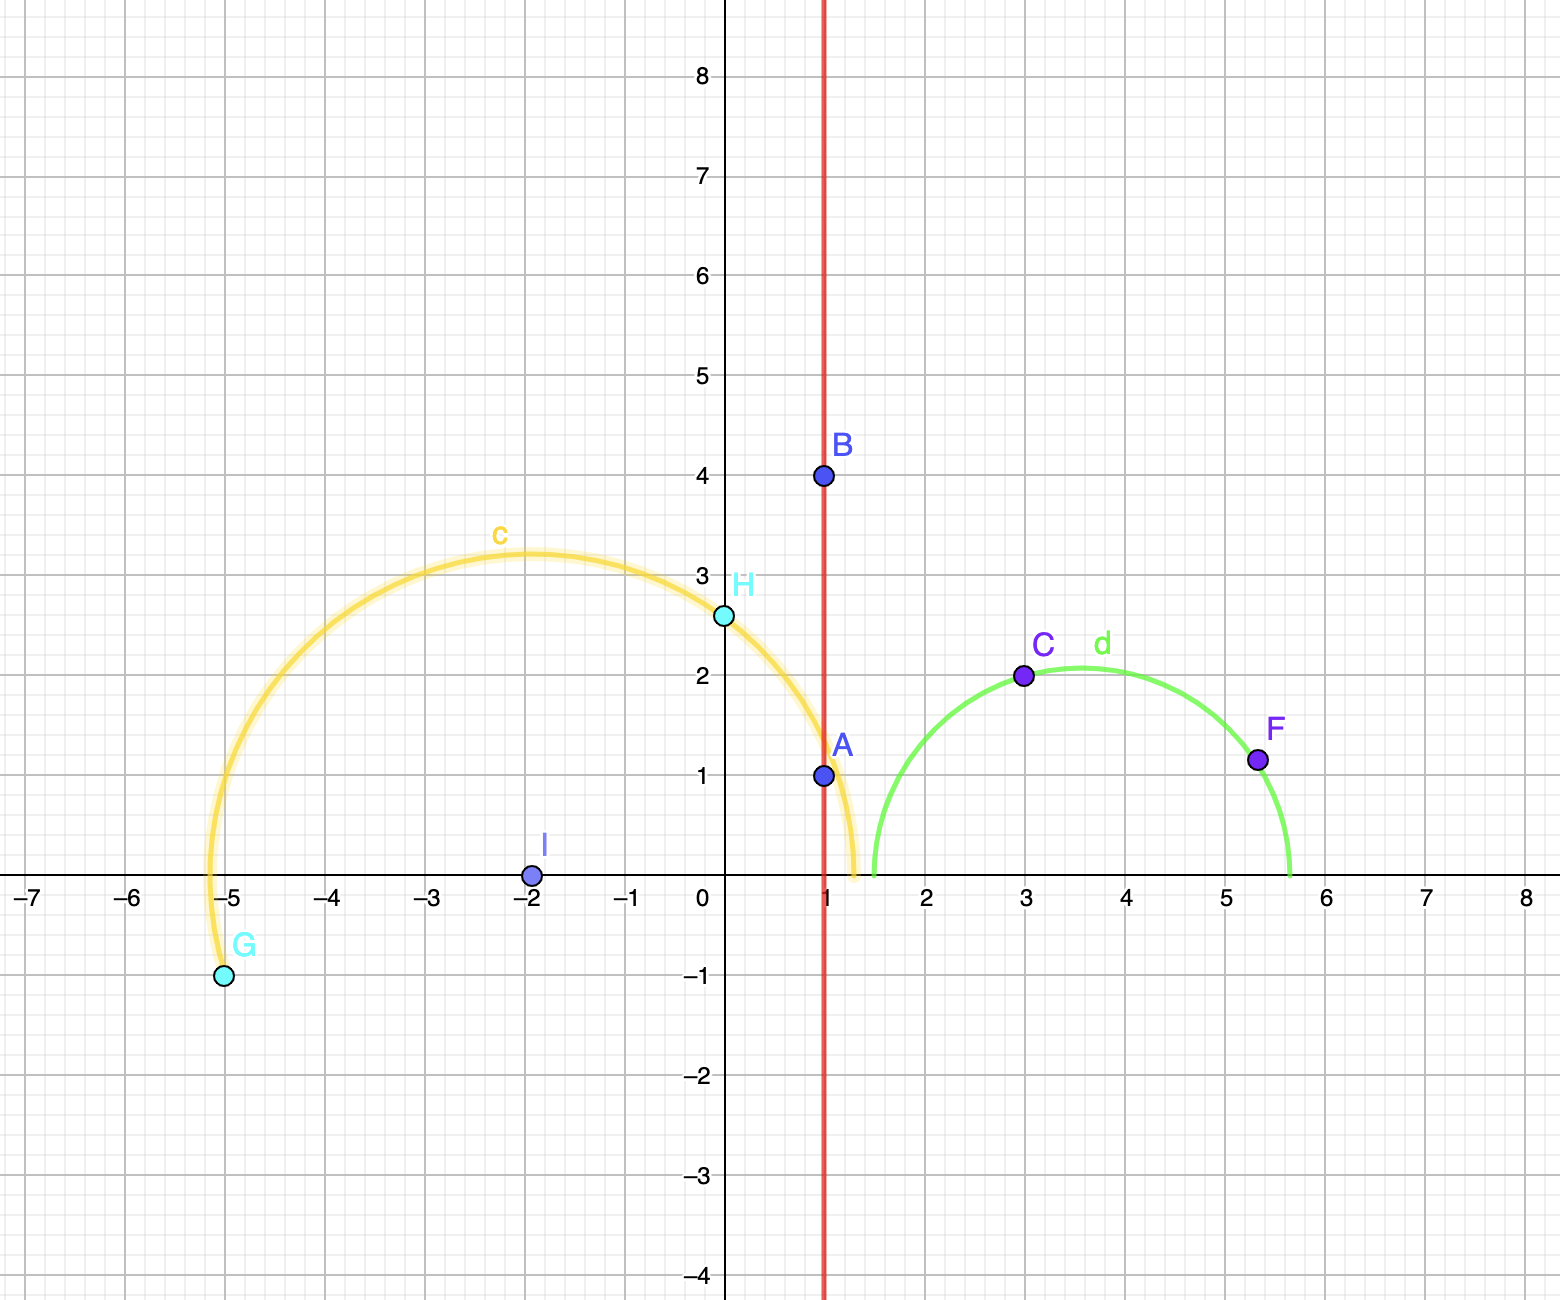
\includegraphics[width=\linewidth]{Bilder/GeodaetischeHyperebene}
	\label{geodaetischeHyperGrafik}
\end{figure}
\end{titleDef}

\begin{titleDef}{Beispiel Bogenlänge parametrisierte imaginäre Achse}
\label{parametrisierungImaginaer}
Hyperbolische geodätische Linien in $X=H^2$ sind genau die Bilder von \hyperref[abstandserhaltend]{abstandserhaltenden} Abbildungen $\gamma:\mathbb{R}\to X$ mit $d_h(\gamma(t_1),\gamma(t_2))$ für den (Bogenlängen-)parameter $t$.\\
Die Parametrisierung der imaginären-/y-Achse nach hyperbolischer \hyperref[bogenlaenge]{Bogenlänge} ist gegeben durch:
$$A_t=\begin{pmatrix}
	e^{\frac{t}{2}}&0\\0&e^{-\frac{t}{2}}
\end{pmatrix},\: \gamma(t)=T_{A_t}(i)=\frac{e^{\frac{t}{2}}i+0}{0i+e^{-\frac{t}{2}}}$$
Damit gilt für $t_2\geq t_1$:
$$d_h(\gamma(t_1),\gamma(t_2))=d_h(e^{t_1}i,e^{t_2}i)=\ln e^{t_2}-\ln e^{t_1}=t_2-t_1$$
damit ist $t$ Bogenlängenparameter.
\end{titleDef}

\newpage
\begin{titleDef}{Abstand von Punkten auf der imaginären Achse}
\label{abstandhyperIm}
Für den Abstand von zwei Punkten $t_1,t_2\in H^2$ die auf der imaginären Achse liegen, d.h
$t_1=\lambda_1i,t_2=\lambda_2i,\lambda_1,\lambda_2\in\mathbb{R}$ gilt:
$$d_h(t_1,t_2)=d_h(\lambda_1i,\lambda_2i)=\lvert ln(\lambda_2)-ln(\lambda_1)\rvert$$
Der einfachheithalber ändere o.B.d.A die Komponenten sodass man den größeren Wert vom kleineren subtrahiert.\\
$$d_h(2i,\frac{1}{2}i)=\lvert\ln(\frac{1}{2})-\ln(2)\rvert=\lvert\ln\left(\frac{\frac{1}{2}}{2}\right)\rvert=\lvert\ln(\frac{1}{4})\rvert=\lvert\ln(1)-\ln(4)\rvert=\lvert0-\ln(4)\rvert=\lvert -2\ln(2)\rvert=2\ln(2)$$
$$d_h(\frac{1}{2}i,2i)=\lvert\ln(2)-\ln(\frac{1}{2})\rvert=\lvert\ln(\frac{2}{\frac{1}{2}})\rvert=\lvert\ln(4)\rvert=\lvert2\ln(2)\rvert=2\ln(2)$$
\end{titleDef}

\begin{titleDef}{Möbiustransformation von geodätischen auf die y-Achse}
Sei $L$ ein euklidischer Halbkrei oder eine Halbgerade in $H^2$, welche die reelle-/x-Achse in einem Punkt $\alpha$ orthogonal schneidet, also ist $L$ gerade eine geodätische Linie in der hyperbolischen Ebene. \\
Dann ist $T(z)=-\frac{1}{z-\alpha}+\beta,\: \beta\in\mathbb{R}$ eine Möbiustransformation die $L$ für ein geeignetes $\beta$ auf die imaginäre-/y-Achse abbildet. d.h es existiert ein $A\in SL(2,\mathbb{R})$ so, dass $T=T_A$. Also gibt es eine Möbiustransformation die eine geodätische Linie auf die imaginäre-/y-Achse abbildet also insbesondere die Punkte die durch diese verbunden werden wobei die Länge zwischen diesen erhalten bleibt, da Möbiustransformationen Isometrien sind.
\end{titleDef}

\begin{titleDef}{Möbiustransformation}
\label{moebiustrans}
Für eine Matrix $$A\in SL(2,\mathbb{R}),\: A=\begin{pmatrix}
	a&b\\c&d
\end{pmatrix},\: det(A)=ad-bc=1$$
definiere die \textbf{Möbiustransformation}
$$T_A:H^2\to H^2;\: z\mapsto\frac{az+b}{cz+d}$$
Es gilt $(T_A)^{-1}=T_{A^{-1}}$\par
Die Möbiustransformation entspricht der Translation und Rotation von euklidischen Ebenen.
\par
Die Möbiustransformationen $\{T_A|\ A\in SL(2,\mathbb{R})\}$ sind \hyperref[Isometrie]{Isometrien} der hyperbolischen Ebene $(H^2,d_h)$ also insbesondere \hyperref[abstandserhaltend]{abstandserhaltend}.\par
Für beliebige Punkte $p,q\in H^2$ existiert eine Isometrie/Möbiustransformation $T_A$ so, dass $T_A(p)=q$.
\end{titleDef}

\begin{titleDef}{Streckung in Hpyerbolischer Ebene}
\label{hyperStreckung}
In der hyperbbolischen Ebene $H^2$ ist die Streckung der Fläche um $\lambda\in\mathbb{R}_{>0}$ ist gegeben durch $s_\lambda:H^2\to H^2$ und wird durch eine \hyperref[moebiustrans]{Möbiustransformation} definiert:
$$s_\lambda=T_A \: \text{für} \: A=\begin{pmatrix}
	\sqrt{\lambda}&0\\0&\frac{1}{\sqrt{\lambda}}
\end{pmatrix}$$
Insondere gibt es also beliebig viele verschiedene streckungen der hyperbolischen Ebene und jede ist eine \hyperref[Isometrie]{Isometrieå} anders als in der euklidischen wo die einzige Streckung die gleichzeitig eine Isometrie ist die Identität ist.
\end{titleDef}



\begin{titleDef}{Hyperbolische Ebene als Metrischer Raum}
\label{hyperToMetrisch}
Nachdem man nun auf der hyperbolischen Ebene $H^2$ mit dem Halbebenen-Modell eine Längenmetrik durch die \hyperref[hyperLaenge]{hypergeometrische Bogenlänge} definiert hat kann man diese nun zu einem \hyperref[MetrischerRaum]{Metrischen Raum} erweitern.\par
Definiere dazu für Punkte $p,q\in H^2$ die Menge $\Omega_{pq}$ als die Menge aller stückweise differenzierbaren \hyperref[kurve]{Kurven} zwischen $p$ und $q$. Dann wird durch
$$d_h(p,q)=\inf\{L_h(c)|\ c\in\Omega_{pq}\}$$
eine Metrik definiert und $(H^2,d_h)$ ist ein \hyperref[MetrischerRaum]{metrischer Raum}
\end{titleDef}

\begin{titleDef}{Unendlicher Rand}
\label{unendlicherRand}
Man kann die hyperbolische Ebene "kompaktifizieren" indem man die reelle-/x-Achse und einen Punkt $\infty$ hinzunimmt: $\overline{H^2}=H^2\cup(\mathbb{R}\cup\{\infty\})$.\\
Das ist zu verstehen als alle Punkte die von einem Punkt $i$ in jeder Richtung unendlich weit entfernt sind.\\
Die Menge $\partial_\infty H^2=\mathbb{R}\cup\infty$ heißt der \textbf{unendliche Rand} von $H^2$.
\end{titleDef}

\begin{titleDef}{hyperbolische Dreiecke}
\label{hyperDreieck}
Ein \textbf{hyperbolisches Dreieck} $\Delta\subset\overline{H^2}$ ist eine \hyperref[konvexPoly]{konvexe} Teilmenge (d.h für zwei Punkte $p,q\in\Delta$ liegt auch das Geradensegment $\overline{pq}$ ganz in $\Delta$) begrenzt von 3 Segmenten von \hyperref[geodaetischPoincare]{geodätischen Linien}, die sich paarweise in Punkten $A,B,C$ den \textbf{Ecken} des Dreiecks schneiden. Die Ecken $A,B,C$ dürfen dabei im \hyperref[unendlicherRand]{unendlichen Rand} $\partial_\infty H^2=\mathbb{R}\cup\{\infty\}$ liegen, die Seiten jedoch nicht.\par
\label{hyperInnenwinkel}
Der \textbf{Innenwinkel} $\varphi$ in einer Ecke $E$ eines Dreickes ist definiert durch die zugrundeliegende \hyperref[riemannMetrik]{Riemannsche Metrik} als die entsprechenden Winkel zwischen den \hyperref[tangentialvektor]{Tangentialvektoren} an die \hyperref[geodaetischPoincare]{geodätischen Linien} wie \hyperref[kennwerteRiemann]{hier} definiert, falls die Ecke in $H^2$ liegt. Falls die Ecke auf dem \hyperref[unendlicherRand]{unendlichen Rand} liegt setzte $\varphi=0$\\
Beachte das der hyperbolische Winkel mit dem euklidischen Winkel übereinstimmt obwohl die hyperbolische Länge sich anders verhält als die euklidische Länge.
\end{titleDef}

\begin{titleDef}{Gauß-Bonnet für hyperbolische Dreiecke}
\label{gaussHyperDreieck}
Der \hyperref[hyperFlaeche]{hyperbolische Flächeninhalt} eines \hyperref[hyperDreieck]{hyperbolischen Dreiecks} $\Delta$ ist durch die drei Innenwinkel $\alpha,\beta,\gamma$ bestimmt und durch $\pi$ beschränkt.
$$0\leq\mu(\Delta)=\pi-(\alpha+\beta+\gamma)$$
Insbesondere ist also $\alpha+\beta+\gamma<\pi$ und $\mu(\Delta)<\pi$
\end{titleDef}
\newpage
\subsection{Einheitskreis-Modell und Gauß-Krümmung}
Wir haben bereits ein Modell für die hypergeometrische Eben gesehen das \hyperref[hyperbolischpoincare]{Poincaré-Halbebenen-Modell}. Hier betrachtet man nun ein alternatives aber offensichtich äquivalentes Modell das \textbf{Einheitskreis-Modell} was "symmetrischer aussieht" als das Halbebenen-Modell

\begin{titleDef}{Von Poincaré zum Einheitskreis}
\label{hyperEinheitskreis}
Sei $D^2=\{(x,y)\in\Rtwo|\ x^2+y^2<1\}=\{z\in\mathbb{C}|\ \lvert z\rvert<1\}$ die \hyperref[einheitskreisscheibeoff]{offene Einheitskreisscheibe}. Die Abbildung
$$M:H^2\subset\mathbb{C}\to D^2\subset\mathbb{C};\: z\mapsto\frac{iz+1}{z+i}$$
ist eine bijektive Abbildung von der \hyperref[hyperbolischpoincare]{Poincaré-Halbebene} $H^2$ in die Einheitskreisscheibe.
\label{einheitskreismetrik}
Analog zur \hyperref[hyperbolischpoincare]{Poincaré-Halbebene} definiert man für das Einheitskreis-Modell eine \hyperref[hyperToMetrisch]{Metrik} 
$$d_h^*(z,w)=d_h(M^{-1})(z),M^{-1}(w))$$
wobei $d_h$ die Metrik der \hyperref[hyperbolischpoincare]{Poincaré-Halbebene} ist also die Länge der kürzesten Kurve die zwei Punkte verbindet.\\
Damit ist nach Konstruktion $M$ automatisch \hyperref[abstandserhaltend]{abstandserhaltend} also eine \hyperref[Isometrie]{Isometrie} also inbesondere eine \hyperref[moebiustrans]{Möbiustransformation} $T_A$ für
$$A=\begin{pmatrix}
	i&1\\1&i
\end{pmatrix}$$
\end{titleDef}

\begin{titleDef}{Metrik des Einheitskreismodells}
\label{metrikEinheitskreis}
$d_h^*$ ist die Längenmetrik die von der \hyperref[riemannMetrik]{Riemmanschen Metrik}
$$(g_{ij}(z))=\left(\frac{4\delta_{ij}}{(1-\lvert z\rvert^2)^2}\right)$$
auf $D^2$ induziert wird. Also ist insbesondere $(D^2,d_h^*)$ ein \hyperref[MetrischerRaum]{Metrischer Raum}.\par
Für $0\leq r<1$ gilt:
$$d_h^*(0,ri)=\ln\left(\frac{1+r}{1-r}\right)$$
\end{titleDef}

\begin{titleDef}{Isometrien des metrischen Raums $(D^2,d_h^*)$}
Neben den \hyperref[moebiustrans]{Möbiustransformationen} $T_A$ die bekannt sind, sind die Rotationen um $0\in D^2$ \hyperref[Isometrie]{Isometrien} im Einheitskreismodell $(D^2,d_h^*)$
\end{titleDef}

\newpage
\begin{titleDef}{Geodätische Linien}
\label{geodaetischeLinienEinheitskreis}
\hyperref[geodaetischeLinie]{Geodätische Linien} also kürzeste Verbindungsstrecken im Einheitskreismodell $(D^2,d_h^*)$ sind :
\begin{itemize}
	\item (geeignet parametrisierte) Geraden durch 0
	\item Alle anderen \hyperref[geodaetischeLinie]{Geodätische Linien} sind euklidische Kreise, die den Einheitskreis orthogonal schneiden.
\end{itemize}
\begin{figure}[h]
	\centering
	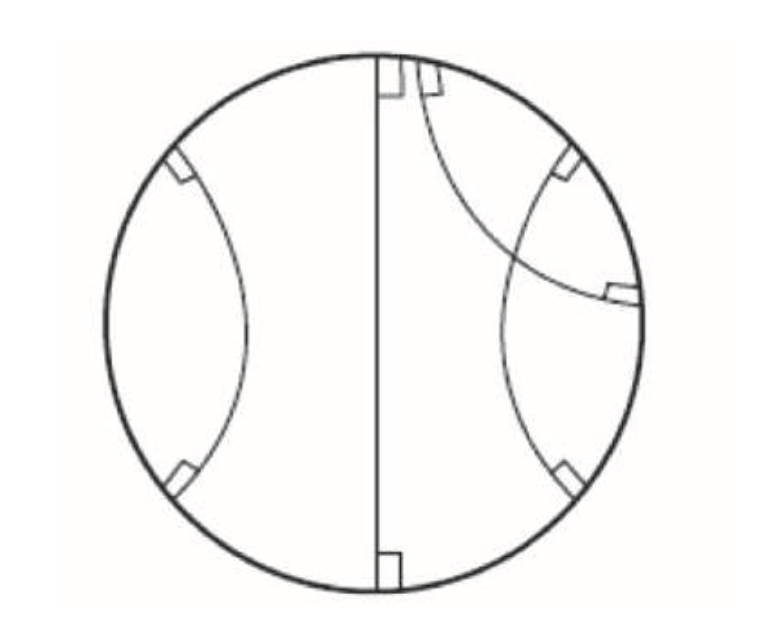
\includegraphics[width=200px]{Bilder/GeodaetischeEinheitskreis}
	\label{geodaetischeHyperEinheitGrafik}
\end{figure}\par
Der \hyperref[unendlicherRand]{unendliche Rand} $\partial_\infty D^2=\mathbb{R}\cup\{\infty\}$ von $D^2$ ist gerade der Einheitskreis $S_1^1$

\end{titleDef}

\begin{titleDef}{hyperbolische Kreis}
\label{hyperKreis}
Der \textbf{hyperbolische Kreis} $S_\varrho(0)$ in $D^2$ mit Zentrum 0 und hyperbolischen Radius (also der Radius gemessen gemäß der \hyperref[hyperLaenge]{hyperbolischen Länge} $L_{h^*}$) ist der euklidische Kreis $S_1^1$ um 0 mit euklidischen Radius r, wobei
$$\varrho=2arctan(r)\Longleftrightarrow r=\tanh(\frac{\varrho}{2})$$
insbesondere gilt $\varrho\to\infty$ für $r\to 1$.\par
Die \hyperref[hyperLaenge]{hyperbolische Länge} des hyperbolischen Kreises $S_\varrho(0)$ ist:
$$L_{h^*}(S_\varrho(0))=2\pi\sinh(\varrho)=2\pi\frac{1}{2}(e^\varrho-e^{-\varrho})\: (\sim\pi e^\varrho \text{ für großes }\varrho)$$
\end{titleDef}

\begin{titleDef}{Gauß-Krümmung}
\label{gausskruemmungEinheitskreis}
Die \hyperref[gausskruemmung]{\textbf{Gauß-Krümmung}} einer hyperbolischen Ebene also von $H^2$ bzw $D^2$ ist konstant $K(p)\cong-1$\par
Reskaliert man die \hyperref[hyperToMetrisch]{hyperbolische Metrik} $d_{h^*}$, setzt also $d_{\tilde{h}}=\lambda d_{h^*}$ für $\lambda\in\mathbb{R}, \lambda>0$ so gilt für die Länge des \hyperref[hyperKreis]{hyperbolischen Kreises}:
$$L_{\tilde{h}}(S_\varrho(0))=2\pi\sinh(\frac{\varrho}{\lambda})$$
daraus folgt für die \hyperref[gausskruemmung]{Gauß-Krümmung} von $(D^2,d_{\tilde{h}})$:
$$K_{\tilde{h}}(p)=-\frac{1}{\lambda^2}=\text{konstant}$$
Durch passende Reskalierungen erhält man also Modelle der hypergeometrischen Ebene mit beliebiger, konstanter negativer Krümmung.\par
Abschließend erhält man also nun für jede reelle Zahl $\alpha\in\mathbb{R}$ eine \hyperref[regFlaeche]{reguläre Fläche} bzw 2-dimensionale \hyperref[diffMannigfaltigkeit]{differenzierbare Mannigfaltigkeit} die genau konstante Krümmung $\alpha$ hat.
\begin{itemize}
	\item Für $\alpha>0$ die \hyperref[ndimsphere]{2-Sphäre} $S_{\frac{1}{\sqrt{\alpha}}}^2$ mit Radius $R=\frac{1}{\sqrt{\alpha}}$
	\item Für $\alpha=0$ die euklidische Ebene
	\item Für $\alpha<0$ die \hyperref[hyperEinheitskreis]{Einheitskreisscheibe} $D^2$ (bzw das isometrische Modell $H^2$ der \hyperref[hyperbolischpoincare]{Poincaré-Halbebene}) mit der Metrik $\frac{1}{\sqrt{\alpha}}d_{h^*}$ bzw $\frac{1}{\sqrt{\alpha}}d_{h}$
\end{itemize}
\end{titleDef}

\end{document}
